
\documentclass[12pt]{article}
%%%%%%%%%%%%%%%%%%%%%%%%%%%%%%%%%%%%%%%%%%%%%%%%%%%%%%%%%%%%%%%%%%%%%%%%%%%%%%%%%%%%%%%%%%%%%%%%%%%%%%%%%%%%%%%%%%%%%%%%%%%%%%%%%%%%%%%%%%%%%%%%%%%%%%%%%%%%%%%%%%%%%%%%%%%%%%%%%%%%%%%%%%%%%%%%%%%%%%%%%%%%%%%%%%%%%%%%%%%%%%%%%%%%%%%%%%%%%%%%%%%%%%%%%%%%
\usepackage{amssymb}
\usepackage{amsfonts}
\usepackage{graphicx}
\usepackage{amsmath}
\usepackage{xkeyval}
\usepackage{tikz}
\usepackage{moretext}
\usepackage{hyperref}
\usepackage{url}

\setcounter{MaxMatrixCols}{10}
%TCIDATA{OutputFilter=LATEX.DLL}
%TCIDATA{Version=5.50.0.2960}
%TCIDATA{<META NAME="SaveForMode" CONTENT="1">}
%TCIDATA{BibliographyScheme=Manual}
%TCIDATA{Created=Tuesday, May 08, 2018 11:08:28}
%TCIDATA{LastRevised=Friday, August 31, 2018 17:35:15}
%TCIDATA{<META NAME="GraphicsSave" CONTENT="32">}
%TCIDATA{<META NAME="DocumentShell" CONTENT="Articles\Literate Programming Article">}
%TCIDATA{Language=American English}
%TCIDATA{CSTFile=Literate Programming Article.cst}

\newtheorem{theorem}{Theorem}
\newtheorem{acknowledgement}[theorem]{Acknowledgement}
\newtheorem{algorithm}[theorem]{Algorithm}
\newtheorem{axiom}[theorem]{Axiom}
\newtheorem{case}[theorem]{Case}
\newtheorem{claim}[theorem]{Claim}
\newtheorem{conclusion}[theorem]{Conclusion}
\newtheorem{condition}[theorem]{Condition}
\newtheorem{conjecture}[theorem]{Conjecture}
\newtheorem{corollary}[theorem]{Corollary}
\newtheorem{criterion}[theorem]{Criterion}
\newtheorem{definition}[theorem]{Definition}
\newtheorem{example}[theorem]{Example}
\newtheorem{exercise}[theorem]{Exercise}
\newtheorem{lemma}[theorem]{Lemma}
\newtheorem{notation}[theorem]{Notation}
\newtheorem{problem}[theorem]{Problem}
\newtheorem{proposition}[theorem]{Proposition}
\newtheorem{remark}[theorem]{Remark}
\newtheorem{solution}[theorem]{Solution}
\newtheorem{summary}[theorem]{Summary}
\newenvironment{proof}[1][Proof]{\textbf{#1.} }{\ \rule{0.5em}{0.5em}}
\input{tcilatex}
\input{litprog.sty}
\begin{document}

\title{The Type System of PLAAY}
\author{Theodore S\ Norvell \\
%EndAName
Electrical and Computer Engineering\\
Memorial University}
\date{\today}
\maketitle

\begin{abstract}
The PLAAY's the thing --- William Shakespear.
\end{abstract}

\tableofcontents

%TCIMACRO{\TeXButton{TeX field}{\section*{List of varables and constants}}}%
%BeginExpansion
\section*{List of varables and constants}%
%EndExpansion

\begin{description}
\item[$e$] expression

\item[$a$] address

\item[$b$] boolean:\ either \textsf{true} or \textsf{false}.

\item[$c$] constness:\ either \textsf{con} or \textsf{loc}.

\item[$d$] declaration

\item[$e$] expression

\item[$f$] field

\item[$h$] context:\ either $\mathrm{L}$ or $\mathrm{R}$

\item[$i,j$] identifier

\item[$k$] natural numbers

\item[$n$] numbers

\item[$m$] members:\ Either expressions or declarations

\item[$p$] primitive types

\item[$q$] type factors

\item[$r,s$] type terms

\item[$t,u,v$] types

\item[$x,y,z$] values
\end{description}

\section{Quick introduction to the PLAAY language}

\subsection{Expressions}

\subsubsection{Abstract syntax}

PLAAY\ is a visual programming language in which the programmer directly
manipulates the abstract syntax of the program. Mostly this document is
about the type system, but this section contains a quick introduction to
some of the abstract syntax for expressions and declarations. Expressions $e$
include%
\begin{eqnarray*}
e &:&:=\mathsf{numberLiteral}\left[ i\right] \\
&\mid &\mathsf{stringLiteral}[i] \\
&\mid &\mathsf{nullLiteral} \\
&\mid &\mathsf{boolLiteral}[b] \\
&\mid &\mathsf{var}[i] \\
&\mid &\mathsf{dot}\left[ i\right] (e) \\
&\mid &\mathsf{tuple}\left( e_{0},e_{1},\ldots ,e_{n-1}\right) \\
&\mid &\mathsf{call}(e_{0},e_{1},\ldots ,e_{n-1}) \\
&\mid &\mathsf{callVar}[i](e_{1},\ldots ,e_{n-1}) \\
&\mid &\lambda \\
&\mid &\mathsf{if}(e,\mathit{seq},\mathit{seq)} \\
&\mid &\mathsf{while}\left( e,\mathit{seq}\right) \\
&\mid &\mathsf{assign}(e_{0},e_{1}) \\
&\mid &\mathsf{loc}\left( e\right) \\
&\mid &\mathsf{objectLiteral}\left( \mathit{seqMember}_{0},\mathit{seqMember}%
_{1},\ldots ,\mathit{seqMember}_{n-1}\right) \\
&\mid &\mathsf{expPH} \\
\lambda &:&:=\mathsf{lambda}(\mathit{params},\mathit{optType,seq})
\end{eqnarray*}%
where $i$ ranges over strings. We have the following additional forms of
trees%
\begin{eqnarray*}
\mathit{params} &:&:=\mathsf{params}\left( d_{0},d_{1},...,d_{n-1}\right) \\
d &:&:=\mathsf{varDecl}[c]\mathsf{(var}[i],\mathit{optType,optExp}) \\
c &:&:=\mathsf{loc}\mid \mathsf{con} \\
\mathit{optType} &:&:=\mathit{type}\mid \mathsf{noType} \\
\mathit{optExp} &:&:=e\mid \mathsf{noExp} \\
\mathit{seq} &:&:=\mathsf{expSeq}\left( m_{0},m_{1},\ldots ,m_{n-1}\right) \\
m &:&:=e\mid d
\end{eqnarray*}

The abstract syntax of of \textit{type} is given in Section \ref%
{sec:type-syntax}.

The set of expressions above roughly corresponds to the language as
implemented in the summer of 2018.

\subsubsection{Informal meaning}

The meanings of most of these constructs are fairly straightforward:

\begin{itemize}
\item number, string, boolean, and null literal evaluate to number, string,
boolean and null values respectively.

\item $\mathsf{var}[i]$ is an occurrence of a variable. Its value is
obtained from the run-time stack. If the variable has not been initialized,
it is an error ---but not a type error.

\item Evaluating $\mathsf{dot}\left[ i\right] (e)$ accesses a field of an
object.

\item Evaluating $\mathsf{tuple}\left( e_{0},e_{1},\ldots ,e_{n-1}\right) $
creates a tuple of values. In the case where $n=1$, its value is the same as
the value of its operand.

\item Evaluating $\mathsf{call}(e_{0},e_{1},\ldots ,e_{n-1})$ applies a
function to an argument. If the argument is not in the domain of the
function, it is a type error. When $e_{0}$ evaluates to a closure with a
declared result type, the value of the function must belong to that type or
is is a type error.

\item $\mathsf{callVar}[i](e_{1},\ldots ,e_{n-1})$\footnote{%
Currently the implementation calls this callWorld. But that is a misnomer
and will be changed.} is just an abbreviation for $\mathsf{call}(\mathsf{var}%
[i],e_{1},\ldots ,e_{n-1})$.

\item Evaluating $\mathsf{lambda}(\mathit{params},\mathit{optType,seq})$
creates a closure. The optional type is the return type. If the return type
is missing, the return type is inferred from the sequence which is its body.

\item Evaluating $\mathsf{assign}(e_{0},e_{1})$ changes the value of one or
more locations in the store. The value of an assign is the empty tuple. The
expression on the left should evaluate to an location value or a tuple of
location values or so on. The expression on the right should evaluate to an
expression of the appropriate type.This distinction between L contexts and R
contexts is discussed more below. Storing a value that does not belong to
the location's type is a type error.

\item Evaluating $\mathsf{if}(e,\mathit{seq},\mathit{seq)}$ evaluates $e$
and then evaluates one of two expression sequences, based on the value of $e$%
. If $e$ evaluates to neither true nor false, it is a type error. Its value
is the value of the chosen sequence.

\item Evaluating $\mathsf{while}\left( e,\mathit{seq}\right) $ evaluates $e$
and then the sequence repeatedly until the expression evaluates to false. If 
$e$ evaluates to neither true nor false, it is a type error. The value of a
loop that terminates is the empty tuple.

\item Evaluating $\mathsf{loc}\left( e\right) $ evaluates $e$ as if it were
on the left side of an assignment. That is $e$ is evaluated in an L context.
The value of $\mathsf{loc}\left( e\right) $ is the same as the value of its
operand evaluated in a L context.

\item Evaluating $\mathsf{objectLiteral}\left( \mathit{seqMember}_{0},%
\mathit{seqMember}_{1},\ldots ,\mathit{seqMember}_{n-1}\right) $ evaluates a
sequence of expressions and declarations (as below). Its value is the stack
frame thus created.

\item $\mathsf{expPH}$ is an expression place-holder. It is used during
editing to hold the place for expressions yet to be added. Evaluating a
place-holder is an error.

\item $\mathsf{expSeq}\left( \mathit{seqMember}_{0},\mathit{seqMember}%
_{1},\ldots ,\mathit{seqMember}_{n-1}\right) $ is evaluated as follows.
First a new stack frame is made, based on the variable declarations.
Initially the variables are uninitialized (or, if you prefer, initialized to
the error value). Second the sequence members are evaluated from left to
right. As the variable declarations are evaluated, the variables become
initialized. The value of the sequence is the value of its last member. If
there are zero members, then the value is the empty tuple. PLAAY\ does not
have a declaration before use rule in order to allow for mutually recursive
function definitions.

\item $\mathsf{varDecl}[c]\mathsf{(var}[i],\mathit{optType,optExp})$
declares a new variable. Evaluating a variable declaration initializes the
variable. If the type is not given, it is inferred from the expression. If
neither is given, the type defaults to the top type. If $c$ is \textsf{con},
the value of the variable is the value of the expression\ (which must not be
missing). If $c$ is $\mathsf{loc}$, a new location is allocated and the
value of the variable is the location; in this case the expression (if
given) is used to initialize the location. It is a type error if the value
of the expression does not belong to the type of the field. The value of a
declaration is the empty tuple.

\item Variable declarations can also appear in parameter lists. In this
case, the value for the variable comes from the corresponding argument in
the case of \textsf{con} variable declarations. For $\mathsf{loc}$
declarations, a new location is created as part of the call and the argument
is used to initialize that location. Initialization expressions can be used
to provide default arguments.
\end{itemize}

\subsubsection{Implicit fetches}

For certain of the expressions listed above, the evaluation of the
expression is immediately followed by an `implicit fetch'. An fetch
operation converts a location to its contents. Implicit fetches only happen
when the value is a location. For example consider an assignment 
\begin{equation*}
\mathsf{assign(var[x],callVar[+](var[y],numberLiteral[1]))}
\end{equation*}%
Suppose the value of $\mathsf{var[x]}$ is a location. There is no implicit
fetch because the expression occurs in an L context. (The left side of an
assignment is an L context.) The expression $\mathsf{var[y]}$ occurs in an R
context. (The operands of a call are R contexts.)\ If $\mathsf{var[y]}$
represents a location, that location is implicitly fetched and the contents
of the location will be the first argument to the function. Implicit
fetching only happens if three things are true:

\begin{itemize}
\item The expression is a \textsf{var} expression, a \textsf{dot}
expression, a \textsf{call} expression or a $\mathsf{callVar}$ expression.

\item The expression occurs in an R context.

\item The value of the expression is a location.
\end{itemize}

Implicit fetcing is done only once: if the result of an implicit fetch is a
location, then that is the result of the expression. For example, suppose $x$
and $y$\ are both variables whose values are locations that hold locations
that hold numbers. Consider $\mathsf{assign(var[x],var[y])}$. The left side
will evaluate to a location that holds a location that holds a number. The
right side will evaluate to a value of the same type, but as implicit fetch
will change that to a location that holds a number. Thus the assignment will
work without error.

As mentioned above, implicit fetches can be suppressed with the $\mathsf{loc}
$ operator; this is in fact its only purpose. Supppose that variable $x$
represents a location that holds a location that holds a number, as above,
and variable $z$ represents a location that holds a number. Consider: 
\begin{equation*}
\mathsf{assign(var[x],loc(var[z]))}
\end{equation*}%
here there is no implicit fetch, so the types of the left and right hand
operands will be as in the previous example. The assignment will work
without error.

A fetch can be forced by calling the identity function. For example, if, as
above, variable $x$ represents a location that holds a location that holds a
number, we could write%
\begin{equation*}
\mathsf{assign(callVar[id](var[x]),numberLiteral[42])}
\end{equation*}%
Since the operand of a call is an R context, $\mathsf{var[x]}$ is implicitly
fetched from; the function's argument (and hence its value) is a location
that holds a number. The call itself occurs in an L context and so there is
no implicit fetch after the call returns. Thus the left side will evaluate
to a location that holds a number. The assignment will work without error.

\subsection{Notation}

Since the abstract syntax can be verbose, I'll sometimes use a sort of
ad-hoc pseudocode. E.g.,%
\begin{equation*}
\lambda \;\mathsf{y}:\mathsf{Loc}[\mathsf{Int}]\cdot \{\;\mathsf{y}:=12\;\}
\end{equation*}%
instead of the abstract syntax%
\begin{equation*}
\mathsf{lambda(}%
\begin{array}[t]{l}
\mathsf{paramList(\;vardecl[con](}%
\begin{array}[t]{l}
\mathsf{var[y],} \\ 
\mathsf{locType(intType),} \\ 
\mathsf{noExp\;)\;)}%
\end{array}
\\ 
\mathsf{noType,} \\ 
\mathsf{exprSeq(assign(}%
\begin{array}[t]{l}
\mathsf{var[y],} \\ 
\mathsf{numberLiteral[12]\;))\;)}%
\end{array}%
\end{array}%
\end{equation*}

\section{An informal introduction to PLAAY's type system}

In PLAAY, values are organized into types. When variables have declared
types, we try to ensure that only values of the given type are associated to
them. This is done through a combination of static (i.e., edit-time\footnote{%
The traditional term is \textquotedblleft compile-time\textquotedblright .
But PLAAY doesn't have a compilation step. Instead errors are reported
through the editor when program is being edited.}) and dynamic (i.e.,
run-time)\ checks. \ The basic principle is to report problems to the user
as soon as possible. Thus we report errors at edit-time when possible.
Errors reported at edit-time may be ignored by the user. That is, the user
may run the program even if errors are being reported. So we still need
run-time checks even for errors that would normally be caught at compile
time. This is in contrast to languages like Java ---where there is limited
need for run-time type checking--- and C ---where run-time checking is
arguably needed, but isn't done.

\subsection{Values}

The following is list of the values in the PLAAY language.

\begin{itemize}
\item String values -- Sequences of 0 or more characters

\item Boolean values.

\item Number values.

\item The null value --- for indicating nullity.

\item The empty tuple.

\item Tuples of 2 or more values.

\item Object values --- Objects comprise named fields that refer to values.

\item Closure values --- These are the result of evaluating lambda
expressions.

\item Built-in function values ---These represent functions implemented in
other languages.

\item Locations --- locations\ are values that hold references to other
values.
\end{itemize}

Let's start the type system by supposing that we have types $\mathsf{String}$%
, $\mathsf{Number}$, $\mathsf{Bool}$, $\mathsf{Null}$. I'll call these types 
\textbf{primitive} types. We'll leave tuples, objects, closures, built-in
functions, and locations to later.

We will use $\limfunc{Val}(t)$ to represent the set of values\footnote{%
The idea that types correspond to sets is likely naive. However, it serves
as a starting point.} that belong to type $t$. For example%
\begin{equation*}
\left\{ 0,1,2,3.14,-42,\ldots \right\} \subseteq \limfunc{Val}(\mathsf{Number%
})
\end{equation*}

\subsection{Extraordinary outcomes}

Usually a computation results in some value. But there are other possible 
\textbf{outcomes}.

\begin{itemize}
\item The error outcome $\blacktriangledown $, representing a computation
that has gone wrong. For example $12\div 0=\blacktriangledown $.

\item A nontermination outcome $\blacktriangle $, representing the result of
a computation that never finishes.
\end{itemize}

We want division, for example, to be such that $x\div y:\mathsf{Number}$
when $x,y:\mathsf{Number}$. Since $12,0:\mathsf{Number}$.

Similarly, we can argue that $\blacktriangledown $ should be in the image of
every type. We want the type of any nonempty expression sequence to be the
type of its last expression. Consider%
\begin{equation*}
\mathsf{ExpSeq}\mathrm{(\mathsf{while}(\mathsf{true},\mathsf{ExpSeq}()),12)}
\end{equation*}

However we don't say that $\blacktriangledown $ or $\blacktriangle $ are
values of type $\mathsf{Number}$, since they aren't values at all; they are
outcomes. We will distinguish between the values of type, written as $%
\limfunc{Val}(t)$ and the possible outcomes of a computation of type $t$,
which we call the type's image, $\func{Im}(t)$. The relationship is simply
that%
\begin{equation*}
\func{Im}(t)=\limfunc{Val}(t)\cup \left\{ \blacktriangledown ,\blacktriangle
\right\}
\end{equation*}

\subsection{The bottom type}

The minimal type we can form is \textquotedblleft bottom\textquotedblright\
notated $\bot $. This type's image contains only $\blacktriangle $ and $%
\blacktriangledown $. We have 
\begin{eqnarray*}
\limfunc{Val}(\bot ) &=&\emptyset \\
\limfunc{Val}(\mathsf{Bool}) &=&\left\{ \mathsf{true},\mathsf{false}\right\}
\end{eqnarray*}%
and 
\begin{equation*}
\limfunc{Val}(\mathsf{Number})=\left\{ 0,1,2,3.14,-42,\ldots \right\}
\end{equation*}%
and so on.

\subsection{Subtypes and soundness}

We write $t<:u$ to mean that $t$ \textbf{is a subtype of} $u$. We can define
this relation on types so that $\bot <:\mathsf{Number}$. In general we want
that, for any types $t$ and $u$%
\begin{equation}
\left( t<:u\right) \Rightarrow \left( \limfunc{Val}(t)\subseteq \limfunc{Val}%
(u)\right)  \tag{Soundness}
\end{equation}%
Furthermore, we want that, for any types $t$, $u$, and $v$,%
\begin{eqnarray}
&&\left. t<:t\right.  \TCItag{Reflexivity} \\
&&\left. \left( t<:u\right) \wedge \left( u<:v\right) \Rightarrow \left(
t<:v\right) \right.  \TCItag{Transitivity}
\end{eqnarray}%
I.e., that subtyping is a preorder.

When $t<:u$ and $u<:t$, we say the types are \textbf{equivalent}. It doesn't
follow that the types are equal. In fact we will regard types to simply be
abstract syntax trees, so two types are equal only when they are written out
exactly the same way. But it does follow that, when $t$ and $u$ are
equivalent, they have the same values. We will write $t\equiv u$ to mean $t$
and $u$ are equivalent.

\subsection{Meets and joins and top}

Given types $t$ and $u$, an upper bound of $t$ and $u$ is any type $v$ such
that $t<:v$ and $u<:v$. We can form the set $U$ of all upper bounds $\left\{
v\mid t<:v\wedge u<:v\right\} $. If there is a $w\in U$ such that $w<:v$ for
all $v$ in $U$, then $w$ is the least upper bound or join of $x$ and $y$, it
is written%
\begin{equation*}
t\sqcup u
\end{equation*}

Dually, we can define the greatest lower bound or meet of $x$ and $y$ as
that member of $w$ of $L=\left\{ v\mid v<:t\wedge v<:t\right\} $ such that $%
v<:w$ for all $v$ in $L$, if such a member exists. We will write it as $%
t\sqcap u$.

We have%
\begin{eqnarray*}
&&t<:t\sqcup u \\
&&u<:t\sqcup u \\
&&t\sqcap u<:t \\
&&t\sqcap u<:u
\end{eqnarray*}

From soundness we can prove that%
\begin{eqnarray*}
\limfunc{Val}(t)\cup \limfunc{Val}(u) &\subseteq &\limfunc{Val}(t\sqcup u) \\
\limfunc{Val}(t\sqcap u) &\subseteq &\limfunc{Val}(t)\cap \limfunc{Val}(u)
\end{eqnarray*}

We will want to arrange that finite joins always exist. We want joins for
example to deal with if-expressions. If $e_{0}:t$ and $e_{1}:u$ and $e_{2}:%
\mathsf{Bool}$ then we want%
\begin{equation*}
\mathsf{if}(e_{2},\mathsf{ExpSeq}(e_{0}),\mathsf{ExpSeq}(e_{2})):t\sqcup u
\end{equation*}%
Also if we catenate a list of $t$ and a list of $u$, we should expect a list
of $t\sqcup u$. The basic intuition for a join is that we use join types
when the type checker can't figure out exactly what type an expression is,
but can narrow it down to either $t$ or $u$ . The two possibilities do not
need to be disjoint. A value could be in both $t$ and $u$; then it is also
in $t\sqcup u$.

%TCIMACRO{\TeXButton{B Figure}{\begin{figure}[tb]}}%
%BeginExpansion
\begin{figure}[tb]%
%EndExpansion

\begin{center}
%TCIMACRO{%
%\TeXButton{TikZPicture}{\begin{tikzpicture}
%\draw (0, 4) node (top) {$\top$ } ;
%
%\draw (0,3) node (bns) {$\mathsf{Bool} \sqcup \mathsf{Number} \sqcup \mathsf{String}$ } ;
%
%\draw (-3,2) node (bn) {$\mathsf{Bool} \sqcup \mathsf{Number}$ } ;
%\draw (0,2) node (bs) {$\mathsf{Bool} \sqcup \mathsf{String}$ } ;
%\draw (3,2) node (ns) {$ \mathsf{Number} \sqcup \mathsf{String}$ } ;
%
%\draw (-2,1) node (b) { $\mathsf{Bool}$ } ;
%\draw (0,1) node (n) { $\mathsf{Number}$ } ;
%\draw (2,1) node (s) { $\mathsf{String}$ } ;
%
%\draw (0,0) node (bot) {$\bot$ } ;
%\draw
%      (top) to  (bns)
%
%     (bns) to (bn)
%     (bns) to (bs) 
%     (bns) to (ns) 
%
%     (bn) to (b)
%     (bn) to (n)
%
%     (bs) to (b)
%     (bs) to (s)
%
%     (ns) to (n)
%     (ns) to (s)
%
%     (b) to (bot)
%     (n) to (bot)
%     (s) to (bot) ;
%\end{tikzpicture}}}%
%BeginExpansion
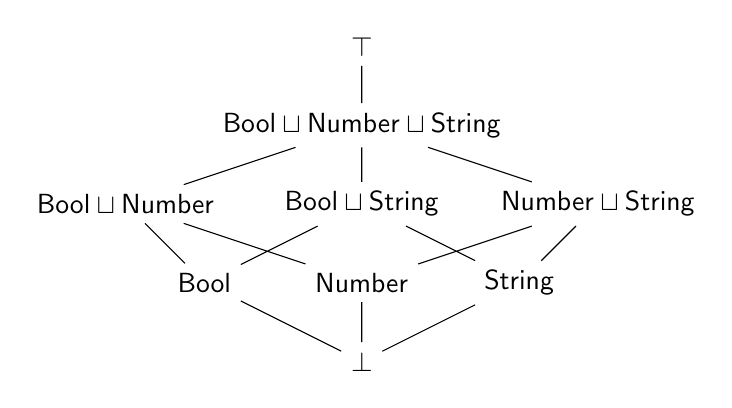
\begin{tikzpicture}
\draw (0, 4) node (top) {$\top$ } ;

\draw (0,3) node (bns) {$\mathsf{Bool} \sqcup \mathsf{Number} \sqcup \mathsf{String}$ } ;

\draw (-3,2) node (bn) {$\mathsf{Bool} \sqcup \mathsf{Number}$ } ;
\draw (0,2) node (bs) {$\mathsf{Bool} \sqcup \mathsf{String}$ } ;
\draw (3,2) node (ns) {$ \mathsf{Number} \sqcup \mathsf{String}$ } ;

\draw (-2,1) node (b) { $\mathsf{Bool}$ } ;
\draw (0,1) node (n) { $\mathsf{Number}$ } ;
\draw (2,1) node (s) { $\mathsf{String}$ } ;

\draw (0,0) node (bot) {$\bot$ } ;
\draw
      (top) to  (bns)

     (bns) to (bn)
     (bns) to (bs) 
     (bns) to (ns) 

     (bn) to (b)
     (bn) to (n)

     (bs) to (b)
     (bs) to (s)

     (ns) to (n)
     (ns) to (s)

     (b) to (bot)
     (n) to (bot)
     (s) to (bot) ;
\end{tikzpicture}%
%EndExpansion
\end{center}

%TCIMACRO{%
%\TeXButton{E Figure}{\caption{Subtype relations between primitive types}\label{fig:prim}
%\end{figure}}}%
%BeginExpansion
\caption{Subtype relations between primitive types}\label{fig:prim}
\end{figure}%
%EndExpansion

It's also good to insist that finite meets exist. For example if we want to
require that a parameter implement two interfaces, we can do so by requiring
that it is in the meet of the two interfaces. Meet types are also useful to
deal with overloaded functions.

Since the only outcomes that $\mathsf{Bool}$ and $\mathsf{Number}$ share are
error and nontermination, we would expect that the meet of these two is $%
\bot $. In general when the meet of two types is $\bot $ we say the types
are disjoint, notated $t%
%TCIMACRO{\TeXButton{disjoint}{\mathrel{\#}}}%
%BeginExpansion
\mathrel{\#}%
%EndExpansion
u$.

We can imagine that there is a type that represents all values, i.e. that
has all values in its image. Call this the \textquotedblleft
top\textquotedblright\ type, denoted by $\top $.

So far we have a picture that looks Figure~\ref{fig:prim} (leaving out a
some atomic types to keep the diagram reasonable).

\subsection{Subtypes of primitive types}

%TCIMACRO{\TeXButton{B Figure}{\begin{figure}[tb]}}%
%BeginExpansion
\begin{figure}[tb]%
%EndExpansion

\begin{center}
%TCIMACRO{%
%\TeXButton{TikZPicture}{\begin{tikzpicture}
%\draw (1, 5) node (top) {$\top$ } ;
%
%\draw (1,4) node (bnum) {$\mathsf{Bool} \sqcup \mathsf{Number}$ } ;
%
%\draw (1,3) node (bint) {$\mathsf{Bool} \sqcup \mathsf{Int}$ } ;
%\draw (-1, 3) node (num) {$\mathsf{Number}$ } ;
%
%\draw (1,2) node (bnat) {$\mathsf{Bool} \sqcup \mathsf{Nat}$ } ;
%\draw (-1,2) node (int) {$ \mathsf{Int}$ } ;
%
%\draw (1,1) node (b) { $\mathsf{Bool}$ } ;
%\draw (-1,1) node (nat) { $\mathsf{Nat}$ } ;
%
%\draw (0,0) node (bot) {$\bot$ } ;
%\draw
%      (top) to  (bnum)
%
%     (bnum) to (bint)
%     (bnum) to (num)
%
%     (num) to (int)
%
%     (bint) to (int)
%     (bint) to (bnat)
%
%     (int) to (nat)
%
%     (bnat) to (nat)
%     (bnat) to (b)
%
%     (b) to (bot)
%     (nat) to (bot) ;
%\end{tikzpicture}}}%
%BeginExpansion
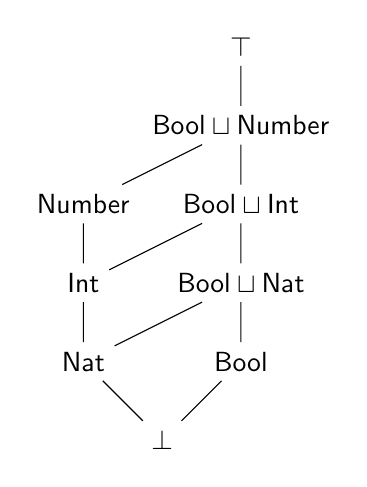
\begin{tikzpicture}
\draw (1, 5) node (top) {$\top$ } ;

\draw (1,4) node (bnum) {$\mathsf{Bool} \sqcup \mathsf{Number}$ } ;

\draw (1,3) node (bint) {$\mathsf{Bool} \sqcup \mathsf{Int}$ } ;
\draw (-1, 3) node (num) {$\mathsf{Number}$ } ;

\draw (1,2) node (bnat) {$\mathsf{Bool} \sqcup \mathsf{Nat}$ } ;
\draw (-1,2) node (int) {$ \mathsf{Int}$ } ;

\draw (1,1) node (b) { $\mathsf{Bool}$ } ;
\draw (-1,1) node (nat) { $\mathsf{Nat}$ } ;

\draw (0,0) node (bot) {$\bot$ } ;
\draw
      (top) to  (bnum)

     (bnum) to (bint)
     (bnum) to (num)

     (num) to (int)

     (bint) to (int)
     (bint) to (bnat)

     (int) to (nat)

     (bnat) to (nat)
     (bnat) to (b)

     (b) to (bot)
     (nat) to (bot) ;
\end{tikzpicture}%
%EndExpansion
\end{center}

%TCIMACRO{%
%\TeXButton{E Figure}{\caption{Adding \textsf{Int} and \textsf{Number}}\label{fig:prim-with-int-and-nat}
%\end{figure}}}%
%BeginExpansion
\caption{Adding \textsf{Int} and \textsf{Number}}\label{fig:prim-with-int-and-nat}
\end{figure}%
%EndExpansion

We introduce two new atomic types: $\mathsf{Int}$ and $\mathsf{Nat}$ with
relationships $\mathsf{Nat}<:\mathsf{Int}<:\mathsf{Number}$. Adding these to
our diagram (but deleting $\mathsf{String}$, to keep the diagram small) we
get Figure~\ref{fig:prim-with-int-and-nat}.

\subsection{Tuple types}

To the set of values, we'll add tuples of values. If $x$ and $y$ are values,
then so are $\left( x,y\right) $, $\left( y,x\right) $, $\left( x,x,y\right) 
$, etc.

A tuple type is one of the following:\ The 0-tuple type, written as $%
\left\langle {}\right\rangle $. A 2-tuple, which is a pair of any types.
written $\left\langle t,u\right\rangle $. And so on for 3, 4, and 5 tuples
etc. We consider tuples of types to be types. Thus the type $\left\langle 
\mathsf{Int},\mathsf{String}\right\rangle $ is a 2-tuple of types and hence
a type. There are no 1-tuple types.

The values of the type $\left\langle {}\right\rangle $ is the set $\left\{
()\right\} $ containing only the empty tuple. The values of $\left\langle 
\mathsf{Int},\mathsf{String}\right\rangle $ contains pairs of values such as 
$\left( 42,\text{\textquotedblleft hello\textquotedblright }\right) $. But
it does not contain pairs with extraordinary outcomes such as $\left(
\blacktriangle ,\blacktriangledown \right) $. The values of $\left\langle
t,u\right\rangle $ is the set 
\begin{equation*}
\limfunc{Val}(t)\times \limfunc{Val}(u\mathsf{)}
\end{equation*}%
And so on for larger tuples. The reason is that, if we try to make a tuple
using erroneous computation, then that is an error. Likewise if we make a
tuple using a nonterminating computation we will get a nonterminating
computation.

It follows that, for any $t$, $\limfunc{Val}(\left\langle t,\bot
\right\rangle )=\emptyset =\limfunc{Val}(\bot )=\limfunc{Val}(\left\langle
\bot ,t\right\rangle )$. So we can expect that $\left\langle t,\bot
\right\rangle \equiv \bot \equiv \left\langle \bot ,t\right\rangle $.

Comparison of tuple types is item-wise, so%
\begin{equation*}
\left( \left\langle t_{0},t_{1}\right\rangle <:\left\langle
u_{0},u_{1}\right\rangle \right) \Leftarrow \left( t_{0}<:u_{0}\wedge
t_{1}<:u_{1}\right)
\end{equation*}%
We cannot make this implication an equivalence because $\left\langle
t_{0},\bot \right\rangle <:\left\langle u_{0},u_{1}\right\rangle $ even if $%
t_{0}<:u_{0}$ is not true.

Tuple types are used to represent types of argument lists when function
calls have other than 1 argument in their argument lists.

\begin{itemize}
\item If a call has one argument in its argument list, that is the argument.
For example a function call $\mathsf{call}(f,12)$ is a call with one
argument, which is of type \textsf{Nat}.

\item If a call has 0 arguments in its argument list, then the argument is
the unit value $()$ and the type of the argument is $\left\langle
{}\right\rangle $. For example a function call $\mathsf{call}(f)$ is
syntactic sugar for $\mathsf{call}(f,())$.

\item And, if the call has two or more arguments in its argument list, they
are tupled to make a single argument. For example, a call $\mathsf{call}%
\left( f,42,\text{\textquotedblleft hello\textquotedblright }\right) $ is
syntactic sugar for a call $\mathsf{call}\left( f,\mathsf{tuple}\left( 42,%
\text{\textquotedblleft hello\textquotedblright }\right) \right) $.
\end{itemize}

\noindent This way all function are officially functions of one argument,
but the syntax makes it easy to pack multiple arguments.

[At some point we might want to think about allowing matching of arguments
to parameters by name. We will also want to deal with omitted arguments and
perhaps variable length argument lists. All of these considerations I'm
going to put off to later.]

Joins of a tuple type and a nontuple type produce a new type that is
different from either of them. So $\left\langle \mathsf{Int},\mathsf{String}%
\right\rangle \sqcup \mathsf{Int}$ is simply itself. The meet of a tuple
type and a nontuple type is $\bot $.

Likewise the join of two tuple types of different lengths is a new type.
E.g., $\left\langle \mathsf{Int},\mathsf{String}\right\rangle \sqcup
\left\langle \mathsf{Int},\mathsf{String},\mathsf{Nat}\right\rangle $ is a
new type that is a supertype of each argument. And the meet of such types is
bottom $\bot $. E.g.,$\left\langle \mathsf{Int},\mathsf{String}\right\rangle
\sqcap \left\langle \mathsf{Int},\mathsf{String},\mathsf{Nat}\right\rangle
\equiv \bot $.

When two tuple types of the same length are joined or meeted, we do the meet
or join itemwise. Thus 
\begin{eqnarray*}
\left\langle t_{0},t_{1}\right\rangle \sqcap \left\langle
u_{0},u_{1}\right\rangle &\equiv &\left\langle t_{0}\sqcap u_{0},t_{1}\sqcap
u_{1}\right\rangle \\
\left\langle t_{0},t_{1}\right\rangle \sqcup \left\langle
u_{0},u_{1}\right\rangle &\equiv &\left\langle t_{0}\sqcup u_{0},t_{1}\sqcup
u_{1}\right\rangle
\end{eqnarray*}

Figure~\ref{fig:tuples} shows some tuple types and their relationships.

%TCIMACRO{\TeXButton{B Figure}{\begin{figure}[tb]}}%
%BeginExpansion
\begin{figure}[tb]%
%EndExpansion

\begin{center}
%TCIMACRO{%
%\TeXButton{TikZPicture}{\begin{tikzpicture}
%\draw (0, 6) node (top) {$\top$ } ;
%
%\draw (0,5) node (tt) {$\langle\top,\top\rangle$ } ;
%\draw (top) to (tt) ;
%
%\draw (-1,4) node (ti) {$\langle\top,\mathsf{Int}\rangle$ } ;
%\draw (+1,4) node (it) {$\langle\mathsf{Int},\top\rangle$ } ;
%\draw (tt) to (ti)   (tt) to (it) ;
%
%\draw (0,3) node (ii) {$\langle\mathsf{Int},\mathsf{Int}\rangle$ } ;
%\draw (-2,3) node (tn) {$\langle\top,\mathsf{Nat}\rangle$ } ;
%\draw (+2,3) node (nt) {$\langle\mathsf{Nat},\top\rangle$ } ;
%\draw (ti) to (tn)   (ti) to (ii)   (it) to (ii)   (it) to (nt) ;
%
%\draw (-1,2) node (in) {$\langle\mathsf{Int},\mathsf{Nat}\rangle$ } ;
%\draw (+1,2) node (ni) {$\langle\mathsf{Nat},\mathsf{Int}\rangle$ } ;
%\draw (tn) to (in)   (ii) to (in)   (ii) to (ni)   (nt) to (ni) ;
%
%\draw (0,1) node (nn) {$\langle\mathsf{Nat},\mathsf{Nat}\rangle$ } ;;
%\draw (in) to (nn)     (ni) to (nn)  ;
%
%\draw (0,0) node (b) {$\bot$ } ;
%\draw (nn) to (b) ;
%
%\end{tikzpicture}}}%
%BeginExpansion
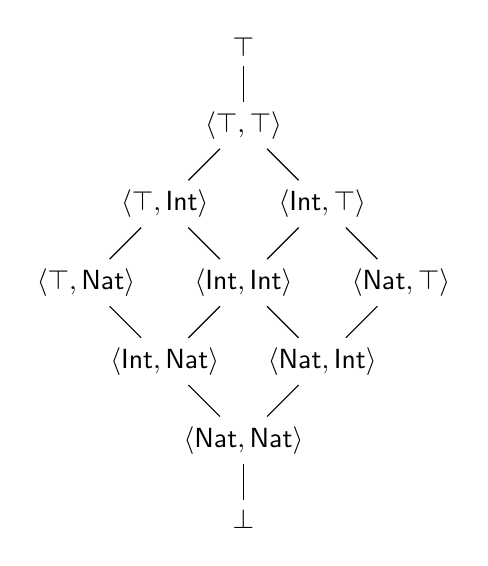
\begin{tikzpicture}
\draw (0, 6) node (top) {$\top$ } ;

\draw (0,5) node (tt) {$\langle\top,\top\rangle$ } ;
\draw (top) to (tt) ;

\draw (-1,4) node (ti) {$\langle\top,\mathsf{Int}\rangle$ } ;
\draw (+1,4) node (it) {$\langle\mathsf{Int},\top\rangle$ } ;
\draw (tt) to (ti)   (tt) to (it) ;

\draw (0,3) node (ii) {$\langle\mathsf{Int},\mathsf{Int}\rangle$ } ;
\draw (-2,3) node (tn) {$\langle\top,\mathsf{Nat}\rangle$ } ;
\draw (+2,3) node (nt) {$\langle\mathsf{Nat},\top\rangle$ } ;
\draw (ti) to (tn)   (ti) to (ii)   (it) to (ii)   (it) to (nt) ;

\draw (-1,2) node (in) {$\langle\mathsf{Int},\mathsf{Nat}\rangle$ } ;
\draw (+1,2) node (ni) {$\langle\mathsf{Nat},\mathsf{Int}\rangle$ } ;
\draw (tn) to (in)   (ii) to (in)   (ii) to (ni)   (nt) to (ni) ;

\draw (0,1) node (nn) {$\langle\mathsf{Nat},\mathsf{Nat}\rangle$ } ;;
\draw (in) to (nn)     (ni) to (nn)  ;

\draw (0,0) node (b) {$\bot$ } ;
\draw (nn) to (b) ;

\end{tikzpicture}%
%EndExpansion
\end{center}

%TCIMACRO{%
%\TeXButton{E Figure}{\caption{Tuples}\label{fig:tuples}
%\end{figure}}}%
%BeginExpansion
\caption{Tuples}\label{fig:tuples}
\end{figure}%
%EndExpansion

\subsection{Function types}

Suppose $t$ is a type and $u$ is a type. Then $t\rightarrow u$ is a function
type.

%TCIMACRO{\TeXButton{B Figure}{\begin{figure}[tb]}}%
%BeginExpansion
\begin{figure}[tb]%
%EndExpansion

\begin{center}
%TCIMACRO{%
%\TeXButton{TikZPicture}{\begin{tikzpicture}
%\draw (0, 8) node (top) {$\top$ } ;
%
%\draw (0,7) node (tt) {$ \bot \rightarrow \top $ } ;
%\draw (top) to (tt) ;
%
%\draw (-1,6) node (ti) {$ \bot \rightarrow \mathsf{Int} $ } ;
%\draw (+1,6) node (it) {$  \mathsf{Nat} \rightarrow \top $ } ;
%\draw (tt) to (ti)   (tt) to (it) ;
%
%
%\draw (-2,5) node (tn) {$ \bot  \rightarrow \mathsf{Nat} $ } ;
%\draw (0,5) node (ii) {$  \mathsf{Nat} \rightarrow \mathsf{Int} $ } ;
%\draw (+2,5) node (nt) {$ \mathsf{Int} \rightarrow \top $ } ;
%\draw (ti) to (tn)   (ti) to (ii)   (it) to (ii)   (it) to (nt) ;
%
%\draw (-3,4) node (tb) {$ \bot \rightarrow \bot $ } ;
%\draw (-1,4) node (in) {$ \mathsf{Nat} \rightarrow \mathsf{Nat} $ } ;
%\draw (+1,4) node (ni) {$ \mathsf{Int} \rightarrow  \mathsf{Int} $ } ;
%\draw (+3,4) node (bt) {$ \top \rightarrow \top $ } ;
%\draw (tn) to (tb) (tn) to (in)   (ii) to (in)   (ii) to (ni)   (nt) to (ni) (nt) to (bt) ;
%
%\draw (-2,3) node (ib) {$ \mathsf{Nat} \rightarrow \bot $ } ;
%\draw (0,3) node (nn) {$ \mathsf{Int} \rightarrow \mathsf{Nat} $ } ;
%\draw (+2,3) node (bi) {$ \top \rightarrow \mathsf{Int} $ } ;
%\draw (tb) to (ib)  (in) to (nn)   (in) to (ib)   (ni) to (nn)   (ni) to (bi)  (bt) to (bi)  ;
%
%\draw (-1,2) node (nb) {$ \mathsf{Int} \rightarrow \bot $ } ;
%\draw (+1,2) node (bn) {$ \top \rightarrow \mathsf{Nat} $ } ;
%\draw (ib) to (nb)   (nn) to (nb)   (nn) to (bn)   (bi) to (bn) ;
%
%\draw (0,1) node (bb) {$ \top \rightarrow \bot $ } ;
%\draw (nb) to (bb)   (bn) to (bb) ;
%
%\draw (0,0) node (b) {$\bot$ } ;
%\draw (bb) to (b) ;
%
%\end{tikzpicture}}}%
%BeginExpansion
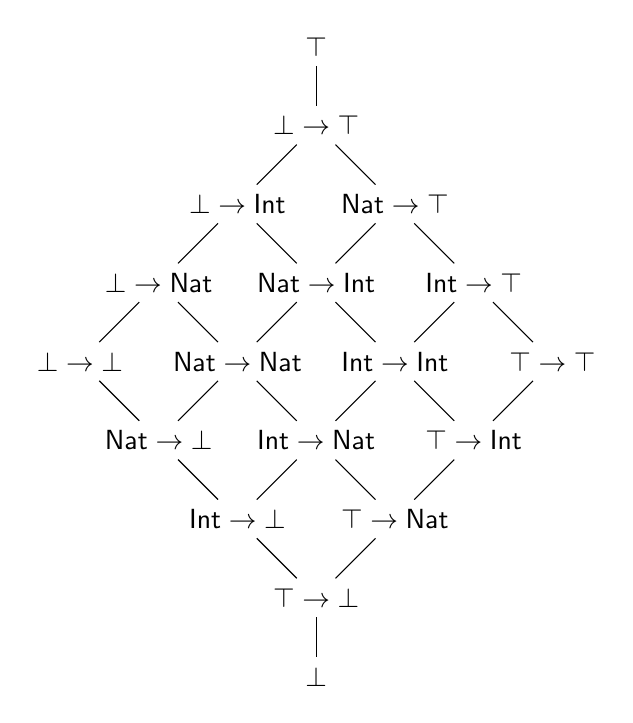
\begin{tikzpicture}
\draw (0, 8) node (top) {$\top$ } ;

\draw (0,7) node (tt) {$ \bot \rightarrow \top $ } ;
\draw (top) to (tt) ;

\draw (-1,6) node (ti) {$ \bot \rightarrow \mathsf{Int} $ } ;
\draw (+1,6) node (it) {$  \mathsf{Nat} \rightarrow \top $ } ;
\draw (tt) to (ti)   (tt) to (it) ;


\draw (-2,5) node (tn) {$ \bot  \rightarrow \mathsf{Nat} $ } ;
\draw (0,5) node (ii) {$  \mathsf{Nat} \rightarrow \mathsf{Int} $ } ;
\draw (+2,5) node (nt) {$ \mathsf{Int} \rightarrow \top $ } ;
\draw (ti) to (tn)   (ti) to (ii)   (it) to (ii)   (it) to (nt) ;

\draw (-3,4) node (tb) {$ \bot \rightarrow \bot $ } ;
\draw (-1,4) node (in) {$ \mathsf{Nat} \rightarrow \mathsf{Nat} $ } ;
\draw (+1,4) node (ni) {$ \mathsf{Int} \rightarrow  \mathsf{Int} $ } ;
\draw (+3,4) node (bt) {$ \top \rightarrow \top $ } ;
\draw (tn) to (tb) (tn) to (in)   (ii) to (in)   (ii) to (ni)   (nt) to (ni) (nt) to (bt) ;

\draw (-2,3) node (ib) {$ \mathsf{Nat} \rightarrow \bot $ } ;
\draw (0,3) node (nn) {$ \mathsf{Int} \rightarrow \mathsf{Nat} $ } ;
\draw (+2,3) node (bi) {$ \top \rightarrow \mathsf{Int} $ } ;
\draw (tb) to (ib)  (in) to (nn)   (in) to (ib)   (ni) to (nn)   (ni) to (bi)  (bt) to (bi)  ;

\draw (-1,2) node (nb) {$ \mathsf{Int} \rightarrow \bot $ } ;
\draw (+1,2) node (bn) {$ \top \rightarrow \mathsf{Nat} $ } ;
\draw (ib) to (nb)   (nn) to (nb)   (nn) to (bn)   (bi) to (bn) ;

\draw (0,1) node (bb) {$ \top \rightarrow \bot $ } ;
\draw (nb) to (bb)   (bn) to (bb) ;

\draw (0,0) node (b) {$\bot$ } ;
\draw (bb) to (b) ;

\end{tikzpicture}%
%EndExpansion
\end{center}

%TCIMACRO{%
%\TeXButton{E Figure}{\caption{Function types}\label{fig:functions}
%\end{figure}}}%
%BeginExpansion
\caption{Function types}\label{fig:functions}
\end{figure}%
%EndExpansion

For example $\mathsf{Int}\rightarrow \mathsf{String}$ represents all
function values (i.e., built-in functions and closures) that, applied to a
value in $\mathsf{Int}$ return a value in $\mathsf{String}$. This includes
impure functions that have side effects. There is no attempt in the type
system to control side effects.

Methods in PLAAY are simply functions that are bound to objects. I\ won't go
into exactly how methods work here. I'll just say that whether a function is
a method or not is not something apparent from its type. This makes it easy
to use methods as call-backs, for example.

The basic idea of subtyping for function types is that they are monotone in
result and anti-monotone in the argument type. For example, suppose we have
a location $x$ of type $\mathsf{Int}\rightarrow \mathsf{Int}$. What values
can we reasonably assign to $x$ besides values that are obviously of type $%
\mathsf{Int}\rightarrow \mathsf{Int}$. Well we can't assign a function of
type $\mathsf{Nat}\rightarrow \mathsf{Int}$, since then a call%
\begin{equation*}
\mathsf{call}(e,\mathsf{numLit}[-1])\qquad \text{,}
\end{equation*}%
where $e$ evaluates to $x$, would cause a run-time error that should have
been caught at design time. But it would be perfectly reasonable to assign a
value of type $\mathsf{Number}\rightarrow \mathsf{Int}$. So we expect that%
\begin{equation*}
\mathsf{Number}\rightarrow \mathsf{Int}<:\mathsf{Int}\rightarrow \mathsf{Int}
\end{equation*}%
On the other hand, it would also make sense to assign $x$ a value of type $%
\mathsf{Int}\rightarrow \mathsf{Nat}$, since any result we get back from
that is going to be an integer. So we expect that 
\begin{equation*}
\mathsf{Int}\rightarrow \mathsf{Nat}<:\mathsf{Int}\rightarrow \mathsf{Int}
\end{equation*}

In general we want%
\begin{equation}
t_{0}\rightarrow u_{0}<:t_{1}\rightarrow u_{1}\text{, if }t_{1}<:t_{0}\text{
and }u_{0}<:u_{1}  \tag{Arrow-Subtype}
\end{equation}%
as illustrated in Figure~\ref{fig:functions}.

\subsubsection{Meets of function types}

The meet of two function types represents overloaded functions.\footnote{%
Currently the only mechanism for overloading is the presence of default
arguments. E.g., an expression%
\begin{equation*}
\mathrm{\lambda con\;x:\mathsf{Nat}:=0\rightarrow \mathsf{Int}\cdot \ldots }
\end{equation*}%
should have both type $\mathsf{Nat\rightarrow Int}$ and $\left\langle
{}\right\rangle \rightarrow \mathsf{Int}$. But other mechanisms may be added
in the future.} For example a function in the image of%
\begin{equation*}
\left( \mathsf{Int}\rightarrow \mathsf{Nat}\right) \sqcap \left( \mathsf{Bool%
}\rightarrow \mathsf{Bool}\right)
\end{equation*}%
is a function that accepts an argument of either type $\mathsf{Int}$ or type 
$\mathsf{Bool}$ and returns a $\mathsf{Nat}$, if the argument is an integer,
and returns a $\mathsf{Bool}$, if the argument is boolean. If the argument
is both an $\mathsf{Int}$ and a $\mathsf{Bool}$ (which would mean an error
or a nontermination) the answer must be in both $\mathsf{Nat}$ and a $%
\mathsf{Bool}$ (which would mean an error or a nontermination). We would
expect this type to be a subtype of each of the following types%
\begin{eqnarray*}
&&\left( \mathsf{Int}\rightarrow \mathsf{Nat}\right) \\
&&\left( \mathsf{Bool}\rightarrow \mathsf{Bool}\right) \\
&&\left( \mathsf{Int}\sqcup \mathsf{Bool}\rightarrow \mathsf{Nat}\sqcup 
\mathsf{Bool}\right) \\
&&\left( \mathsf{Int}\sqcap \mathsf{Bool}\rightarrow \mathsf{Nat\sqcap Bool}%
\right)
\end{eqnarray*}

Certain built-in functions are best described by meets. For example, the
addition function could be described by an infinite meet. 
\begin{eqnarray*}
&&\left( \left\langle {}\right\rangle \rightarrow \mathsf{Nat}\right) \\
&&\sqcap \left( \mathsf{Nat}\rightarrow \mathsf{Nat}\right) \sqcap \left( 
\mathsf{Int}\rightarrow \mathsf{Int}\right) \sqcap \left( \mathsf{Number}%
\rightarrow \mathsf{Number}\right) \\
&&\sqcap \left( \left\langle \mathsf{Nat},\mathsf{Nat}\right\rangle
\rightarrow \mathsf{Nat}\right) \sqcap \left( \left\langle \mathsf{Int},%
\mathsf{Int}\right\rangle \rightarrow \mathsf{Int}\right) \sqcap \left(
\left\langle \mathsf{Number},\mathsf{Number}\right\rangle \rightarrow 
\mathsf{Number}\right) \\
&&\sqcap \left( \left\langle \mathsf{Nat},\mathsf{Nat},\mathsf{Nat}%
\right\rangle \rightarrow \mathsf{Nat}\right) \sqcap \left( \left\langle 
\mathsf{Int},\mathsf{Int},\mathsf{Int}\right\rangle \rightarrow \mathsf{Int}%
\right) \sqcap \left( \left\langle \mathsf{Number},\mathsf{Number},\mathsf{%
Number}\right\rangle \rightarrow \mathsf{Number}\right) \\
&&\sqcap \cdots
\end{eqnarray*}%
This is an example of an infinite meet that should exist. For technical
reasons this paper assumes only that finite meets exist. For practical
purposes, we could cut off the type of addition after some large number of
arguments. There are also no doubt ways around the technical limitations in
the special cases that we need.

\paragraph{Function meets with the same argument type}

If we have a function with both type $\mathsf{Int}\rightarrow \mathsf{Int}$
and $\mathsf{Int}\rightarrow \mathsf{Bool}$, we can conclude that supplying
the function with an $\mathsf{Int}$ will result in an object that is both a $%
\mathsf{Int}$ and a $\mathsf{Bool}$. And since these result types are
disjoint, this function call can only end in error or nontermintion. It
seems reasonable to guess that%
\begin{equation*}
\left( \mathsf{Int}\rightarrow \mathsf{String}\right) \sqcap \left( \mathsf{%
Int}\rightarrow \mathsf{Bool}\right) \equiv \left( \mathsf{Int}\rightarrow
\bot \right)
\end{equation*}%
and more generally that 
\begin{equation*}
\left( t\rightarrow u_{0}\right) \sqcap \left( t\rightarrow u_{1}\right)
\equiv \left( t\rightarrow u_{0}\sqcap u_{1}\right)
\end{equation*}%
But we are not forced to this conclusion. From the (arrow-subtype) rule, we
can see that%
\begin{equation*}
\left. \left( t\rightarrow u_{0}\sqcap u_{1}\right) <:\left( t\rightarrow
u_{2}\right) \right. \text{if and only if }u_{0}\sqcap u_{1}<:u_{2}
\end{equation*}%
Taking $u_{2}=u_{0}$ we get%
\begin{equation*}
\left( t\rightarrow u_{0}\sqcap u_{1}\right) <:\left( t\rightarrow
u_{0}\right)
\end{equation*}%
and likewise%
\begin{equation*}
\left( t\rightarrow u_{0}\sqcap u_{1}\right) <:\left( t\rightarrow
u_{1}\right)
\end{equation*}%
From the last two and that $a<:b$ and $a<:c$ implies $a<:b\sqcap c$ we get
that%
\begin{equation*}
\left( t\rightarrow u_{0}\sqcap u_{1}\right) <:\left( t\rightarrow
u_{0}\right) \sqcap \left( t\rightarrow u_{1}\right)
\end{equation*}%
The question then is: is it also the case that 
\begin{equation*}
\left( t\rightarrow u_{0}\right) \sqcap \left( t\rightarrow u_{1}\right)
<:\left( t\rightarrow u_{0}\sqcap u_{1}\right) \qquad \text{?}
\end{equation*}%
From the proposed definition of image above, it seems the right thing to do
to decree that this is true.

\paragraph{Function meets with disjoint argument types}

When the argument types are disjoint as in $\left( \mathsf{Int}\rightarrow 
\mathsf{Nat}\right) \sqcap \left( \mathsf{Bool}\rightarrow \mathsf{Int}%
\right) $ we can see that this should be a subtype of $\left( \mathsf{Int}%
\sqcap \mathsf{Bool}\rightarrow \mathsf{Nat}\sqcap \mathsf{Int}\right) $
which is the same as $\mathsf{\bot }\rightarrow \mathsf{Nat}$. If we insist
that functions are monotonic in the sense that they always map error
arguments to error results and nonterminating arguments to nonterminating
results, we might go further and expect that $\left( \mathsf{Int}\rightarrow 
\mathsf{Nat}\right) \sqcap \left( \mathsf{Bool}\rightarrow \mathsf{Int}%
\right) $ is a subtype of $\mathsf{\bot }\rightarrow \mathsf{\bot }$. To
obtain, this we would need a rule that $t\rightarrow u<:\mathsf{\bot }%
\rightarrow \mathsf{\bot }$, for all types $t$ and $u$.

\paragraph{Function meets with common result types}

Consider $\left( \mathsf{Bool}\rightarrow \mathsf{String}\right) \sqcap
\left( \mathsf{Nat}\rightarrow \mathsf{String}\right) $. The two argument
types are disjoint. We might expect that 
\begin{equation*}
\left( \mathsf{Bool}\rightarrow \mathsf{String}\right) \sqcap \left( \mathsf{%
Nat}\rightarrow \mathsf{String}\right) \equiv \left( \mathsf{Bool}\sqcup 
\mathsf{Nat}\rightarrow \mathsf{String}\right)
\end{equation*}%
and more generally that 
\begin{equation*}
\left( t_{0}\rightarrow u\right) \sqcap \left( t_{1}\rightarrow u\right)
\equiv \left( t_{0}\sqcup t_{1}\rightarrow u\right)
\end{equation*}%
From (arrow-subtype) we get $\left( t_{0}\rightarrow u\right) <:\left(
t_{0}\sqcup t_{1}\rightarrow u\right) $ and we also have $\left(
t_{1}\rightarrow u\right) <:\left( t_{0}\sqcup t_{1}\rightarrow u\right) $.
From this we get 
\begin{equation*}
\left( t_{0}\rightarrow u\right) \sqcap \left( t_{1}\rightarrow u\right)
<:\left( t_{0}\sqcup t_{1}\rightarrow u\right)
\end{equation*}%
However to get the other half of the equivalence, we must decree that%
\begin{equation*}
\left( t_{0}\sqcup t_{1}\rightarrow u\right) <:\left( t_{0}\rightarrow
u\right) \sqcap \left( t_{1}\rightarrow u\right)
\end{equation*}

\subsubsection{Joins of function types}

[to be done]

\subsection{Field types}

We now consider objects. An object is a collection of fields. Each field has
a name (unique within the object), a type, and a value.

If $i$ is an identifier and $t$ is a type, then $i\colon t$ is a \textbf{%
field type}. The image of this type is all objects that have a field named $%
i $ of type $t$. These objects can have other fields too.

Consider $\mathsf{a\colon Bool}$ this type's image includes the objects%
\begin{equation*}
\left\{ \mathsf{a\colon Bool}\mapsto \mathsf{true}\right\}
\end{equation*}%
and%
\begin{equation*}
\left\{ \mathsf{a\mathsf{\colon Bool}\mapsto true},\mathsf{b\mathsf{\colon }%
Nat\mapsto 12}\right\}
\end{equation*}%
The latter of these is also in the images of $\mathsf{b}$\textsf{$\colon $}$%
\mathsf{Nat}$, $\mathsf{b}$\textsf{$\colon $}$\mathsf{Int}$, and $\mathsf{a}$%
\textsf{$\colon $}$\mathsf{Bool\sqcap b}$\textsf{$\colon $}$\mathsf{Int}$.

We can see then that the following laws seem reasonable 
\begin{equation*}
i\colon t<:i\colon u\text{, if }t<:u
\end{equation*}%
and 
\begin{equation*}
i\colon t\sqcap u<:i\colon t
\end{equation*}%
for any $u$.

A field type or a meet of field types is called an \textbf{interface type}.
These correspond roughly to interfaces in languages like Java. The type $%
\mathsf{a}$\textsf{$\colon $}$\mathsf{Bool\sqcap b}$\textsf{$\colon $}$%
\mathsf{Int}$ represents all objects that have both a field named
\textquotedblleft \textsf{a}\textquotedblright\ that contains only values in
the image of type $\mathsf{Bool}$ and a field \textquotedblleft \textsf{b}%
\textquotedblright\ that contains only values in the image of type $\mathsf{%
Int}$.

[Suppose, for a moment, we consider that for each individual string there is
a corresponding type, so $\left. \text{\textquotedblleft }\mathsf{a}\text{%
\textquotedblright }<:\mathsf{String}\right. $ and $\limfunc{Val}\left( 
\text{\textquotedblleft }\mathsf{a}\text{\textquotedblright }\right)
=\left\{ \text{\textquotedblleft }\mathsf{a}\text{\textquotedblright }%
\right\} $. Then $\mathsf{a}$\textsf{$\colon $}$\mathsf{Bool}$ can be
considered to be equivalent to \textquotedblleft $\mathsf{a}$%
\textquotedblright $\rightarrow \mathsf{Bool}$. I'm not yet willing to take
this step.]

Sequences can be thought of as a combination of a function and a length
field. Thus (Following Reynolds [[1988]]) $\mathsf{Seq}[t]$ is a synonym for 
$\left( \mathsf{Nat}\rightarrow t\right) \sqcap \left( \mathsf{length:Nat}%
\right) $. We have $\mathsf{Seq}[t]<:\mathsf{Seq}[u]$ whenever $t<:u$.

\subsection{Locations}

\textbf{A short comment on wording:} In PLAAY ---or at least in this
document--- we use the word \textbf{variable} in the mathematical sense of a
name for a value. Variables may be parameters, local variables, or fields of
objects.\ (In fact, since activation frames are simply objects, all three
kinds of variable are fields.) Anyway for the lifetime of a variable its
\textquotedblleft value\textquotedblright\ does not change, except to change
from uninitialized to initialized. In order to accommodate imperative
programming, we need assignment. In PLAAY, the thing we assign to is a 
\textbf{location}. Locations can be thought of as addresses that index a
store. Assignment alters the store. Locations are themselves considered
values and so we can use variables to name locations. Earlier documentation
may use these words differently. \textbf{end comment}

If we have an assignment command $a:=e$, where $a$ is a $\mathsf{Number}$
location, $e$ could be of type $\mathsf{Number}$ or $\mathsf{Int}$ or $%
\mathsf{Nat}$. If we think of $a:=$ as a function $f$ so that $a:=e$ can be
written as $f(e)$, we find that $f$ is a function of type $\mathsf{Number}%
\rightarrow \left\langle {}\right\rangle $.\footnote{%
As mentioned above, functions can have side effects.}

At first I considered three approaches to locations:

\begin{itemize}
\item Following Reynolds' [[1988]] design for Forsythe, we can think of a
location of type $t$ as being an object of type $t\sqcap \left( t\rightarrow
\left\langle {}\right\rangle \right) $. Then $a:=e$ is literally an
abbreviation for $a(e)$. Under this approach we define $\mathsf{Loc}%
[t]\equiv t\sqcap \left( t\rightarrow \left\langle {}\right\rangle \right) $%
. Thus $\mathsf{Loc}[t]<:t$, for all $t$.

\item A second approach is to think of a location of type $t$ as being an
object of type $t\sqcap \mathsf{set}\colon \left( t\rightarrow \left\langle
{}\right\rangle \right) $ with $a:=e$ being an abbreviation for $a.\mathsf{%
set}\left( e\right) $. Under this approach we define $\mathsf{Loc}[t]\equiv
t\sqcap \mathsf{set}\colon \left( t\rightarrow \left\langle {}\right\rangle
\right) $ (or at least $\mathsf{Loc}[t]<:t$) $\mathsf{Loc}[t]<:t\sqcap 
\mathsf{set}\colon \left( t\rightarrow \left\langle {}\right\rangle \right) $%
).

\item A third approach is to think of a location of type $t$ as being an
object of type $\mathsf{get}\colon \left( \left\langle {}\right\rangle
\rightarrow t\right) \sqcap \mathsf{set}\colon \left( t\rightarrow
\left\langle {}\right\rangle \right) $ with the application of $.\mathsf{get}
$ being implicit. In this approach the assignment $a:=e$ is an abbreviation
for $a.\mathsf{set}\left( e\right) $. With this approach we define $\mathsf{%
Loc}[t]\equiv \mathsf{get}\colon \left( \left\langle {}\right\rangle
\rightarrow t\right) \sqcap \mathsf{set}\colon \left( t\rightarrow
\left\langle {}\right\rangle \right) $. In this case it is not true that $%
\mathsf{Loc}[t]<:t$. This means that at certain places in the code (called R
contexts), locations will need to be dereferenced.
\end{itemize}

We take an approach similar to the third. $\mathsf{Loc}[t]$ is a class that
implements $\mathsf{get}\colon \left( \left\langle {}\right\rangle
\rightarrow t\right) \sqcap \mathsf{set}\colon \left( t\rightarrow
\left\langle {}\right\rangle \right) $.

We can abbreviate $\mathsf{get}\colon \left( \left\langle {}\right\rangle
\rightarrow t\right) $ as $\mathsf{Source}[t]$ and $\mathsf{set}\colon
\left( t\rightarrow \left\langle {}\right\rangle \right) $ as $\mathsf{%
Acceptor}[t]$. So%
\begin{equation*}
\mathsf{Loc}[t]<:\mathsf{Source}[t]\sqcap \mathsf{Acceptor}[t]
\end{equation*}

The rationale for rejecting the first two approaches is this. Both these
approaches have the seeming advantage that $\mathsf{Loc}[t]<:t$. This seems
to simplify, for example, the type checking of assignments.\ For example if $%
x$ and $y$ are both expressions of type $\mathsf{Loc}[\mathsf{Int}]$ then
the assignment $x:=y$ will type check for the same reason that the
assignment $x:=12$ type checks, i.e., that the type of the right-side is a
subtype of $\mathsf{Nat}$. This can be summed up in the type checking rule%
\begin{equation*}
\dfrac{x:v\qquad y:t\qquad v<:\mathsf{Acceptor}[u]\qquad t<:u}{%
x:=y:\left\langle {}\right\rangle }
\end{equation*}%
(Where $\mathsf{Acceptor}[u]$ is defined as $u\rightarrow \left\langle
{}\right\rangle $ for the first choice and as $\mathsf{set}\colon \left(
t\rightarrow \left\langle {}\right\rangle \right) $ for the second and
third.) So up to now everything looks good. But consider an expression $z$
of type $\mathsf{Loc}[\mathsf{Loc}[\mathsf{Int}]]$. This is a subtype of $%
\mathsf{Loc}[\mathsf{Int}]$ which is a subtype of $\mathsf{Int}$ and so, by
transitivity $\mathsf{Loc}[\mathsf{Loc}[\mathsf{Int}]]$ is a subtype of $%
\mathsf{Int}$ and we are forced to conclude that $x:=z$ should also type
check. This would be OK if the PLAAY followed the lead of Gedanken
[[Reynolds, 1970]] and made it part of the semantics of assignments that the
right-hand side is repeatedly fetched from until a nonlocation is found.
However that would make assignment to variables of type $\mathsf{Loc}[%
\mathsf{Loc}[t]]$ impossible (Gedanken has a second assignment operator for
the purpose of allowing assignments of locations. Forsythe does not have
locations that can hold locations.)\ The intention in PLAAY is that the
right hand side of an assignment will be fetched from only once if possible
and otherwise not at all. In PLAAY, our example $x:=z$ does not type check
since there is no $u$ such that $\mathsf{Loc}[\mathsf{Int}]<:\mathsf{Acceptor%
}[u]$ and either $\mathsf{Loc}[\mathsf{Loc}[\mathsf{Int}]]<:u$ or $\mathsf{%
Loc}[\mathsf{Loc}[\mathsf{Int}]]<:\mathsf{Source}[u]$; this is what we want.
The price is that the rules for type checking assignments are a bit more
complex.

In the previous paragraph, I've used assignment as an example. Similar
remarks apply to operands of other operators, such as the call operator. In
assignment, the left operand is said to be in an L context. The right
operand is said to be in an R context. Expressions in an R context may be
evaluated slightly differently from expressions in an L context; var, dot
and call expressions in an R context are evaluated in two phases; in the
first, the expression is evaluated as if it were in an L context. In the
second, if the result of the first phase is a source, the source is fetched
from, otherwise the result is just the result of the first phase. Every
expression in a program can be considered to be in an R context or an L
context. Arguments to calls are in an R context, as are the first operands
of `if' and `while' expressions and the bodies of lambda expressions. The
operands of the tupling operation inherit their context from the tuple
operation itself. For example in the tree%
\begin{equation*}
\mathsf{assign(tuple(var[a],var[b]),tuple(var[c],numberLiteral[12]))}
\end{equation*}%
the first tuple is in an L context and so its children are also; the second
tuple is in an R context and so its children are also.

\subsubsection{Some consequences}

We have that $\mathsf{Loc}[t]\equiv \mathsf{Loc}[u]$ is true when $t\equiv u$%
.

When $t\not\equiv u$ and neither is equivalent to $\bot $, we should expect
that on semantic grounds $\mathsf{Loc}[t]\ $and $\mathsf{Loc}[u]$ are
disjoint, i.e. that the intersection of their value is empty. This can be
justified on semantic grounds as follows. Suppose $t\not\equiv u$. Then
there may be at least one value in the image of $t$ that is not in the image
of $u$ or the other way around. Without loss of generality, suppose $x$ is
in the image $t$ and not in the image of $u$. Of course $x$ is a value.
Consider an ordinary member $y$ that is in the image of $\mathsf{Loc}\left[ u%
\right] $ which has a set field which gives an error when applied to $x$
and, more importantly, does not update the contents of the location. $y$
should not be in the image of $\mathsf{Loc}[t]$. Now consider any ordinary
member $z$ of the image of $\mathsf{Loc}[t]$. After we set $z$ to $x$ it has
a value that is not in $u$, a location that might hold a value not in $u$
should not be in the image of $\mathsf{Loc}\left[ u\right] $.

What about the case that $t\not\equiv u$, but one of $t$ and $u$ is
equivalent to $\bot $. Suppose, without loss of generality that $t\equiv
\bot $ and $u\not\equiv \bot $. An value of type $\mathsf{Loc}[t]$ would be
an address of a part of the store that can not hold any values. Do such
values exist?\ We don't have to decide yet.

\begin{itemize}
\item Suppose we decide that $\mathsf{Loc}[t]$ has no values. Then we have
that $\limfunc{Val}(\mathsf{Loc}[t])=\emptyset .$So $\limfunc{Val}(\mathsf{%
Loc}[t])\cap \limfunc{Val}(\mathsf{Loc}\left[ u\right] )=\emptyset $.

\item On the other hand, if we decide that there are values in $\limfunc{Val}%
(\mathsf{Loc}[t])$, they can not accept values of $\limfunc{Val}(u)$ and so
are not in $\mathsf{Loc}\left[ u\right] $. Any ordinary values of $\mathsf{%
Loc}\left[ u\right] $ would be able to store and later produce ordinary
values of $\limfunc{Val}(u)$, which an ordinary value in $\limfunc{Val}(%
\mathsf{Loc}[t])$ would not be able to do. And so, again, we conclude that $%
\limfunc{Val}(\mathsf{Loc}[t])\cap \limfunc{Val}(\mathsf{Loc}\left[ u\right]
)=\emptyset $.
\end{itemize}

Either way, if $t\not\equiv u$ then the intersection of their values should
be empty.

\subsubsection{Aliasing}

By admitting variables as values, we open a can of worms, which is aliasing.
However this can was, in fact, already open in the Winter 2018
implementation of PLAAY. (In PLAAY an object can end up as part of the stack
chain and so an assignment to a location $a$ might also change a field $p.a$
in an object accessed through a pointer. Likewise an assignment to $p.a$
might change location $a$.) As this genie is already partway out of the
bottle the choice is whether to find a way to stuff it back in, or to let it
out all the way. Java stuffs the genie back in the bottle by not allowing
any aliasing between stack variables and stack variables nor between stack
variables and heap variables. C++ allows unfettered aliasing. Allowing this
aliasing may make automated verification more tricky. On the other hand
Occam's razor seems to lead us to location types.

On the plus side, pass-by-reference parameters (reference parameters for
C++ers, var parameters for Pascal fans)\ are now perfectly natural; for
example, we have a type $\mathsf{Loc}[t]\rightarrow u$.\footnote{%
There is a catch here because at the call site side we typically need to
suppress the normal value conversion. E.g., if $x$ is a $\mathsf{Loc(Int)}$
and $f$ is a $\mathsf{Loc[Int]\rightarrow Int}$ then $\mathsf{call(}f,%
\mathsf{var}[x]\mathsf{)}$ will normally pass an $\mathsf{Int,}$leading to a
type error. So either we need to do something fancy on semantics of the
call, or we need for the caller to indicate which parameters are passed by
reference. I\ don't want to do anything in the semantics that causes types
to changes the meaning of a legitimate program.\ (Technically we want an
erasure property in which the types of a correct program can be erased
without changing its meaning.) That leaves it to the programmer to mark
reference parameters at the call site. For this we have the operator \textsf{%
loc} whose operand is an L-context. Then the call would look like $\mathsf{%
call(}f,\mathsf{loc}\left( \mathsf{var}[x]\right) \mathsf{)}$. I\ don't mind
this, as it makes the code more readable and the semantics simple.} Mutable
fields in interfaces also make sense for example, $\mathsf{f}\colon \mathsf{%
Loc}[t]$.

It is tempting to think that location declarations are just abbreviations
for constant declarations. For example we might expect that%
\begin{equation*}
\mathbf{loc}\;\mathsf{x}:\mathsf{Int:=12}
\end{equation*}%
is just an abbreviation for%
\begin{equation*}
\mathsf{x}:\mathsf{Loc}[\mathsf{Int}]:=\mathsf{12}
\end{equation*}%
but this is not right, since the type of 12 is $\mathsf{Nat}$ and $\mathsf{%
Nat}$ is not a subtype of $\mathsf{Loc}[\mathsf{Int}],$so the latter has a
type error, while th former should not. A location declaration creates (at
runtime)\ a new location while a constant declaration simply gives a name to
a value. We can think of%
\begin{equation*}
\mathbf{loc}\;\mathsf{x}:\mathsf{Int:=12}
\end{equation*}%
as an abbreviation for%
\begin{equation*}
\mathsf{x}:\mathsf{Loc}[\mathsf{Int}]:=\mathsf{new\;Loc}(\mathsf{12)}
\end{equation*}%
where $\mathsf{Loc}$ is a constructor of locations.\footnote{%
The construction $\mathsf{new\;Loc}(\mathsf{-)}$ looks a bit like the
construction $\mathsf{loc}\left( \mathsf{-}\right) $ proposed in an earlier
foot note but they are different $\mathsf{new\;Loc}(\mathsf{-)}$ evaluates
its operand for value (i.e., its operand is an R-context) and wraps a
location around the value. The construction $\mathsf{loc}\left( \mathsf{-}%
\right) $ evaluates its operand for location. For example if $x$ is a $%
\mathsf{Loc(Int)}$, then $\mathsf{new\;Loc}(x\mathsf{)}$ is a new $\mathsf{%
Loc(Int)}$ that initially shares the same value as $x$, but $\mathsf{loc}%
\left( x\right) $ simply evaluates to original location named $x$ itself.}

For similar reasons, the pass-by-reference parameters of a function are
usually written as constant declarations. For example this lambda expression%
\begin{equation}
\lambda \;\mathsf{y}:\mathsf{Loc}[\mathsf{Int}]\cdot \{\;\mathsf{y}:=12\;\}
\label{eq:assign12}
\end{equation}%
has type $\mathsf{Loc}[\mathsf{Int}]\rightarrow \left\langle {}\right\rangle 
$. The lambda expression%
\begin{equation}
\lambda \;\mathbf{loc}\;\mathsf{y}:\mathsf{Int}\cdot \{\;\mathsf{y}:=\mathsf{%
y}+1\;;\;y\;\}\qquad \text{,}  \label{eq:inc0}
\end{equation}%
on the other hand, has type$\;\mathsf{Int}\rightarrow \mathsf{Int}$. It is a
pure function with no side effects. The fact that the parameter is declared
as a location is purely a matter that is internal to the function's
implementation. The function (\ref{eq:inc0}) has the same type and does the
same thing (although in a slightly different way) as the function%
\begin{equation*}
\lambda \;\mathsf{y}:\mathsf{Int}\cdot \{\;\mathsf{y}+1\;\}
\end{equation*}%
The lambda expression%
\begin{equation*}
\lambda \;\mathbf{loc}\;\mathsf{y}:\mathsf{Loc}[\mathsf{Int}]\cdot \{\;%
\mathsf{y}:=12\;\}
\end{equation*}%
would have the same type as (\ref{eq:assign12}), but it has a type error in
the assignment: the type of $y$ is $\mathsf{Loc}[\mathsf{Loc[Int]}]$ and the
type of $12$ is $\mathsf{Nat}$ and $\mathsf{Nat}$ is not a subtype of $%
\mathsf{Loc[Int]}$. A correct, but gratuitously complex, equivalent to (\ref%
{eq:assign12}) is 
\begin{equation*}
\lambda \;\mathbf{loc}\;\mathsf{y}:\mathsf{Loc}[\mathsf{Int}]\cdot \{\;%
\mathsf{id(y)}:=12\;\}
\end{equation*}%
where $\mathsf{id}$ is the identity function.

Arrays can be thought of as sequences of locations. A declaration%
\begin{equation*}
a:\;:=\;\mathbf{new\;}\mathsf{Array[Int}](10)
\end{equation*}%
declares a new variable of type $\mathsf{Seq[Loc[Int]]}$. Consider the
assignment $a(i):=b(i)$ where $a$ and $b$ are both arrays. The call on the
left side returns a location. The call on the right side also returns a
location, but this location is implicitly fetched.

\subsection{Classes}

Classes are blueprints for objects. A class is a type, but it is more than a
type in the sense that there are things we can do with classes that we can
not do with other types. For example we can use a class to create new
objects.

I'm going to ignore classes for now and come back to them later. When I come
back to them we will find that a class $k$ that defines a field $i$ of type $%
t$ will be such that $i\colon t<:k$.

\subsection{Named types and recursion}

As a convenience to the programmer, we should allow complex types to be
abbreviated with a name and that name to be used in place of the type.
However we will not allow recursion. (At least not yet.) For example a
declaration like this%
\begin{equation*}
\mathbf{typename}\;\mathsf{fred}=(\mathsf{head}:\mathsf{int}\sqcap \mathsf{%
tail}:\mathsf{fred)}
\end{equation*}%
which introduces a new name \textsf{fred} and then uses that name in its
definition, would not be allowed.

\section{Formalizing the type system}

\subsection{Abstract syntax for types\label{sec:type-syntax}}

[To be done]

\subsection{Types}

We will define the types of PLAAY to be all trees finitely generated by the
following abstract grammar which defines types%
\begin{eqnarray*}
t,u,v::= &&r \\
&\mid &t\sqcup u \\
&\mid &\bot
\end{eqnarray*}%
type terms%
\begin{eqnarray*}
r,s::= &&q \\
&\mid &r\sqcap s \\
&\mid &\top
\end{eqnarray*}%
type factors%
\begin{eqnarray*}
q::= &&p \\
&\mid &\left\langle {}\right\rangle \mid \left\langle
t_{0},t_{1}\right\rangle \mid \left\langle t_{0},t_{1},t_{3}\right\rangle
\mid \cdots \\
&\mid &t\rightarrow u \\
&\mid &i\colon t \\
&\mid &\mathsf{Loc}[t]
\end{eqnarray*}%
and primitive types%
\begin{equation*}
p::=\mathsf{Bool\mid String\mid Number}\mid \mathsf{Int}\mid \mathsf{Nat}%
\mid \mathsf{Null}
\end{equation*}%
where $i$ is any identifier. This formalization ignores the use of
identifiers as types, since that is easily dealt with in other ways. Note
that we assume that types are always in join normal form; that is a type
always has its joins outside of meets; $(\mathsf{Bool}\sqcup \mathsf{Int}%
\mathrm{)}\sqcap \mathsf{Null}$ is not a type according to the above
grammar, but we can rewrite it as a type $\left( \mathsf{Bool}\sqcap \mathsf{%
Null}\right) \sqcup \left( \mathsf{Int}\sqcap \mathsf{Null}\right) $.

\subsection{The length of types}

For types factors, we can define a length of the type factor%
\begin{eqnarray*}
\#\left\langle {}\right\rangle &=&0 \\
\#p &=&\#\left( t\rightarrow u\right) =\#\left( i\colon t\right) =\#\mathsf{%
Loc}[t]=1 \\
\#\left\langle t_{0},t_{1}\right\rangle &=&2 \\
\#\left\langle t_{0},t_{1},t_{3}\right\rangle &=&3 \\
&&\cdots
\end{eqnarray*}

\subsection{Subtypes}

We wish to formally define the subtype relation $t<:u$. We do that by first
defining a relationship between finite sets of types. We'll define%
\begin{equation*}
\Theta <:\Delta
\end{equation*}%
where $\Theta $ and $\Delta $ are finite sets of types and then define $t<:u$
as $\left\{ t\right\} <:\left\{ u\right\} $. The intended interpretation is
that $\Theta <:\Delta $ should hold only if the intersection\footnote{%
The interssection of $0$ sets here is considered to be the universe of all
values. This universe $V$ and will be defined in a later section along with
the $\limfunc{Val}$ function.} of the values of types in $\Theta $ is
contained in the union of values in types in $\Delta $:%
\begin{equation*}
\Theta <:\Delta \qquad \Rightarrow \qquad \dbigcap\limits_{t\in \Theta }%
\limfunc{Val}(t)\subseteq \dbigcup\limits_{u\in \Delta }\limfunc{Val}(u)
\end{equation*}%
This is soundness. Completeness of the subtype relation is the converse
implication. Fans of logic may recognize that $\Theta <:\Delta $ is
analogous to a sequent in the sequent calculus.

We can define the relation $\Theta <:\Delta $ as the least relation that
obeys the following rules. \ In these rules and below, we abbreviate a
singleton set $\left\{ t\right\} $ by its sole occupant $t$ and $\Theta \cup
\left\{ t\right\} $ with $\Theta ,t$.

\begin{itemize}
\item Reflexive rule%
\begin{equation*}
\Theta <:\Theta
\end{equation*}

\item Subset rules%
\begin{equation*}
\frac{\Theta <:\Delta }{\Theta <:\Delta \cup \Pi }
\end{equation*}%
and%
\begin{equation*}
\frac{\Theta <:\Delta }{\Theta \cup \Pi <:\Delta }
\end{equation*}

\item Cut Rule%
\begin{equation*}
\frac{\Theta <:\Delta \cup \Pi \qquad \Pi \cup \Theta <:\Delta }{\Theta
<:\Delta }
\end{equation*}

\item Top and bottom rules:%
\begin{equation*}
\bot <:\Delta \qquad \frac{\Theta <:\emptyset }{\Theta <:\bot }
\end{equation*}%
and%
\begin{equation*}
\Theta <:\top \qquad \frac{\emptyset <:\top }{\top <:\Delta }
\end{equation*}

\item Primitive rules%
\begin{equation*}
\mathsf{Int}<:\mathsf{Number}\qquad \mathsf{Nat}<:\mathsf{Number}\qquad 
\mathsf{Nat}<:\mathsf{Int}
\end{equation*}

\item Tuple rule. For tuples of equal length%
\begin{equation*}
\frac{t_{0}<:u_{0}\qquad t_{1}<:u_{1}\qquad \cdots }{\left\langle
t_{0},t_{1},...\right\rangle <:\left\langle u_{0},u_{1},...\right\rangle }
\end{equation*}

\item Function rule%
\begin{equation*}
\frac{u_{0}\mathsf{<:}t_{0}\qquad t_{1}\mathsf{<:}u_{1}}{\left(
t_{0}\rightarrow t_{1}\right) <:\left( u_{0}\rightarrow u_{1}\right) }
\end{equation*}

\item Field rules%
\begin{equation*}
\frac{t<:u}{i\colon t<:i\colon u}\text{ }
\end{equation*}

\item Location rules%
\begin{equation*}
\frac{t<:u\qquad u<:t}{\mathsf{Loc}[t]<:\mathsf{Loc}[u]}
\end{equation*}%
and%
\begin{equation*}
\frac{\mathsf{get}\colon \left( \left\langle {}\right\rangle \rightarrow
t\right) ,\mathsf{set}\colon \left( t\rightarrow \left\langle
{}\right\rangle \right) <:\Delta }{\mathsf{Loc}[t]<:\Delta }
\end{equation*}

\item Meet rules%
\begin{equation*}
\frac{r_{0},r_{1}<:\Delta }{r_{0}\sqcap r_{1}<:\Delta }
\end{equation*}%
and%
\begin{equation*}
\frac{\Theta <:u_{0}\qquad \Theta <:u_{1}}{\Theta <:u_{0}\sqcap u_{1}}
\end{equation*}

\item Join rules%
\begin{equation*}
\frac{\Theta <:u_{0},u_{1}}{\Theta <:u_{0}\sqcup u_{1}}
\end{equation*}%
and%
\begin{equation*}
\frac{t_{0}<:\Delta \qquad t_{1}<:\Delta }{t_{0}\sqcup t_{1}<:\Delta }
\end{equation*}
\end{itemize}

The following additional rules allow us to prove disjointness. A\ set of
types $\Theta $ is \textbf{disjoint} if $\Theta <:\emptyset $. As set of
types $\Theta $ is \textbf{pair-wise disjoint} if for every two different
types $t,u\in \Theta $, $\left\{ t,u\right\} <:\emptyset $.

\begin{itemize}
\item Length disjointness rule. This rule relies on the definition of length
given above.%
\begin{equation*}
\frac{\#q_{0}\neq \#q_{1}}{q_{0},q_{1}<:\emptyset }
\end{equation*}

\item Primitive disjointness rules.%
\begin{eqnarray*}
\mathsf{Bool},\mathsf{Number} &<&:\emptyset \\
\mathsf{Bool},\mathsf{String} &<&:\emptyset \\
\mathsf{Bool},\mathsf{Null} &<&:\emptyset \\
\mathsf{Number},\mathsf{String} &<&:\emptyset \\
\mathsf{Number},\mathsf{Null} &<&:\emptyset \\
\mathsf{String},\mathsf{Null} &<&:\emptyset
\end{eqnarray*}

\item Tuple disjointness rules%
\begin{equation*}
\frac{t_{0},u_{0}<:\emptyset }{\left\langle t_{0},t_{1}\right\rangle
,\left\langle u_{0},u_{1}\right\rangle <:\emptyset }\qquad \frac{%
t_{1},u_{1}<:\emptyset }{\left\langle t_{0},t_{1}\right\rangle ,\left\langle
u_{0},u_{1}\right\rangle <:\emptyset }
\end{equation*}%
and%
\begin{equation*}
\frac{t_{0},u_{0}<:\emptyset }{\left\langle t_{0},t_{1},t_{2}\right\rangle
,\left\langle u_{0},u_{1},u_{2}\right\rangle <:\emptyset }\qquad \frac{%
t_{1},u_{1}<:\emptyset }{\left\langle t_{0},t_{1},t_{2}\right\rangle
,\left\langle u_{0},u_{1},u_{2}\right\rangle <:\emptyset }\qquad \frac{%
t_{2},u_{2}<:\emptyset }{\left\langle t_{0},t_{1},t_{2}\right\rangle
,\left\langle u_{0},u_{1},u_{2}\right\rangle <:\emptyset }
\end{equation*}%
and so on.

\item Other disjointness rules. Recall that $p$ ranges over primitive types.%
\begin{eqnarray*}
&&p,\left( t\rightarrow u\right) <:\emptyset \\
&&p,\left( i:t\right) <:\emptyset \\
&&p,\mathsf{Loc}[t]<:\emptyset \\
&&\left( t\rightarrow u\right) ,\mathsf{Loc}[t]<:\emptyset
\end{eqnarray*}

\item \lbrack [Perhaps we need a rule that location types are disjoint from
objects that don't implement the location type's interface.]]
\end{itemize}

\subsection{Values and semantics of types}

In this section we give a semantics for types. It uses sets rather than
domains. I\ think this is adequate for the purpose of showing the subtype
relation sound and complete and providing a basis for dynamic and static
type checking. The use of sets for semantics is common in logic and I\ think
it works here for the same reasons it works there.\footnote{%
The semantics given here might not be adequate as a basis for providing a
semantics to the expressions of the language. But that is not my current
purpose. That is a bridge to be crossed later. The semantics of expressions
will use either an operational approach or the predicative programming
approach of Hehner and Kassios; perhaps both. An operational semantics is
obviously useful for guiding (or confirming)\ the implementation of
language. An predicative semantics would provide the basis for contracts and
(automated) proofs of programs. Having both would provide a chain from
design-by-contract to the implementation.}

\subsubsection{Values}

Values are trees following this abstract grammar%
\begin{eqnarray*}
x,y,z\in \mathcal{V} &:&:=\mathsf{boolv}\left( b\right) \\
&\mid &\mathsf{stringv}\left( \mathit{str}\right) \\
&\mid &\mathsf{numberv}\left( n\right) \\
&\mid &\mathsf{tuplev}\left( x_{0},x_{1},\ldots x_{k}\right) \\
&\mid &\mathsf{nullv} \\
&\mid &\mathsf{obv}\left( f_{0},f_{1},...f_{k}\right) \\
&\mid &\mathsf{locv}\left( t,a\right) \\
&\mid &\mathsf{closurev}\left( \lambda ,\eta ,t\rightarrow u,a\right) \\
&\mid &\mathsf{builtinv(}t\rightarrow u,a) \\
f &:&:=\mathsf{field}(i,t,a) \\
\lambda &:&:=\mathsf{lambda}(\mathit{params},\mathit{optType,seq})
\end{eqnarray*}%
where: $b$ is a boolean in the set $\left\{ \mathsf{true,false}\right\} $; $%
\mathit{str}$ is a string from a set of strings $\mathcal{S}$; $n$ is a
rational number from a set of rational numbers $\mathcal{Q}$\footnote{$%
\mathcal{Q}$ could be the set of all rational numbers or some subset that is
conveniently represented on the computer; in the current implementation it
is the set of numbers that javascript can represent and so includes positive
and negative infinities and various NaN values in addition to a subset of
the rationals.}; $t$ and $u$ are types; $a$ is an address from a countable
and infinite set of addresses $\mathcal{A}$; $\eta $ is an environment,
which is a finite sequence of values each of which is an \textsf{obv}; and $%
i $ is an identifier from a countable, infinite, totally ordered set of
identifiers $\mathcal{I}$. In any $\mathsf{obv}$, no two fields may have the
same identifier and we restrict the fields of an $\mathsf{obv}$ to being in
order by identifier.\ In \textsf{tuplev}, the number of values must not be 1.

Values are trees in the sense that there are no loops. Equality of values is
completely straight forward. Two values are equal if they are the same tree.%
\footnote{%
In contrast to most OOPLs there is (technically) no object identity. However
fields do have identity, since they have addresses. Thus if we evaluate$%
\bigskip $ the expression
\par
\begin{equation*}
\begin{array}[t]{l}
\mathsf{objectLiteral(\;vardecl[con](}%
\begin{array}[t]{l}
\mathsf{var[a],} \\ 
\mathsf{intType,} \\ 
\mathsf{numberLiteral[123]\;)\;)}%
\end{array}%
\end{array}%
\end{equation*}%
twice we will get unequal objects since we will get objects with unequal
fields, since the semantics of field creation demands that a new address is
used for each field creation. This is an artifact of the evaluation
semantics and not baked in to the structure of values.}

We'll also assume that each address is associated with exactly one type. For
example%
\begin{equation*}
x=\mathsf{locv}\left( t_{0},a\right) \wedge y=\mathsf{locv}\left(
t_{1},a\right) \Rightarrow t_{0}=t_{1}\wedge \mathsf{locv}\left(
t_{0},a\right) =\mathsf{locv}\left( t_{1},a\right)
\end{equation*}%
We can imagine that each element of $\mathcal{A}$ is associated with just
one type and that each time we create a location, we are sure to pick an
address associated with the appropriate type. Similarly for fields,
closures, and built-ins.

Note that location values exist even if the type is equivalent to $\bot $.
In practice such values are not useful and we can make it a dynamic or
static error to create one. But in terms of defining our set of values we
will say that they exist. A similar comment applies to fields.

\subsubsection{Semantics of types}

For each type $t$, we'll define a set of values $\limfunc{Val}(t)$. We
define 
\begin{equation*}
\func{Im}(t)=\limfunc{Val}(t)\cup \left\{ \blacktriangle ,\blacktriangledown
\right\} 
\end{equation*}

Next we define the Val function.%
\begin{eqnarray*}
\limfunc{Val}\left( \top \right) &=&\mathcal{V} \\
\limfunc{Val}\left( \bot \right) &=&\emptyset \\
\limfunc{Val}\left( r\sqcap s\right) &=&\limfunc{Val}\left( r\right) \cap 
\limfunc{Val}\left( s\right) \\
\limfunc{Val}\left( t\sqcup u\right) &=&\limfunc{Val}\left( t\right) \cup 
\limfunc{Val}\left( u\right)
\end{eqnarray*}

For tuple types we have

\begin{eqnarray*}
\limfunc{Val}(\left\langle {}\right\rangle ) &=&\left\{ \mathsf{tuplev()}%
\right\} \\
\limfunc{Val}(\left\langle t_{0},t_{1}\right\rangle ) &=&\left\{ \mathsf{%
tuplev}(x_{0},x_{1})\in \mathcal{V}\mid x_{0}\in \limfunc{Val}(t_{0})\wedge
x_{1}\in \limfunc{Val}(t_{1})\right\} \\
&&\ldots
\end{eqnarray*}%
Since the members of $\mathcal{V}$ are trees, we can not have tuple values
that contain themselves.

For function types we have%
\begin{eqnarray*}
\limfunc{Val}\left( t_{0}\rightarrow u_{0}\right) &=&\left\{ \mathsf{closurev%
}\left( t_{1}\rightarrow u_{1},\lambda ,\eta ,a\right) \in \mathcal{V}\mid 
\limfunc{Val}(t_{0})\subseteq \limfunc{Val}(t_{1})\wedge \limfunc{Val}%
(u_{1})\subseteq \limfunc{Val}(u_{0})\right\} \\
&&\cup \left\{ \mathsf{builtinv}\left( t_{1}\rightarrow u_{1},a\right) \in 
\mathcal{V}\mid \limfunc{Val}(t_{0})\subseteq \limfunc{Val}(t_{1})\wedge 
\limfunc{Val}(u_{1})\subseteq \limfunc{Val}(u_{0})\right\}
\end{eqnarray*}

For fields%
\begin{eqnarray*}
\limfunc{ObVal}\left( i:t\right)  &=&\left\{ \mathsf{obv}\left( \ldots ,%
\mathsf{field}(j,u,a),\ldots \right) \in \mathcal{V}\mid i=j\wedge \limfunc{%
Val}(u)\subseteq \limfunc{Val}(t)\right\}  \\
\limfunc{Val}\left( i:t\right)  &=&\left\{ 
\begin{array}{lll}
\limfunc{ObVal}\left( i:t\right) \cup \left\{ \mathsf{locv}(u,a)\mid 
\limfunc{Val}(u\rightarrow \left\langle {}\right\rangle )\subseteq \limfunc{%
Val}(t)\right\}  & \qquad  & \text{if }i=\mathsf{set} \\ 
\limfunc{ObVal}\left( i:t\right) \cup \left\{ \mathsf{locv}(u,a)\mid 
\limfunc{Val}(u)\subseteq \limfunc{Val}(t)\right\}  &  & \text{if }i=\mathsf{%
get} \\ 
\limfunc{ObVal}\left( i:t\right)  &  & \text{otherwise}%
\end{array}%
\right. 
\end{eqnarray*}

For location types%
\begin{equation*}
\limfunc{Val}\left( \mathsf{Loc}[t]\right) =\left\{ \mathsf{locv}(u,a)\mid 
\limfunc{Val}(t)=\limfunc{Val}(u)\right\}
\end{equation*}

For primitive types we have%
\begin{eqnarray*}
\limfunc{Val}(\mathsf{Bool}) &=&\left\{ \mathsf{boolv}\left( \mathsf{true}%
\right) ,\mathsf{boolv}\left( \mathsf{false}\right) \right\} \\
\limfunc{Val}(\mathsf{String}) &=&\left\{ \mathsf{stringv}\left( str\right)
\mid str\in \mathcal{S}\right\} \\
\limfunc{Val}(\mathsf{Number}) &=&\left\{ \mathsf{numberv}\left( n\right)
\mid n\in \mathcal{Q}\right\} \\
\limfunc{Val}(\mathsf{Int}) &=&\left\{ \mathsf{numberv}\left( n\right) \mid
n\in \mathcal{Q}\wedge n\text{ is an integer}\right\} \\
\limfunc{Val}(\mathsf{Nat}) &=&\left\{ \mathsf{numberv}\left( n\right) \mid
n\in \mathcal{Q}\wedge n\text{ is a nonnegative integer}\right\} \\
\limfunc{Val}(\mathsf{Null}) &=&\left\{ \mathsf{nullv}\right\}
\end{eqnarray*}

\subsubsection{Soundness}

At this point we have formally defined types, subtyping, and images; so we
can ask the questions of whether the subtyping relation is sound

\begin{equation}
\forall t,u\cdot \left( t<:u\right) \Rightarrow \left( \limfunc{Val}%
(t)\subseteq \limfunc{Val}(u)\right)  \tag{Soundness}
\end{equation}%
and complete%
\begin{equation}
\forall t,u\cdot \left( \limfunc{Val}(t)\subseteq \limfunc{Val}(u)\right)
\Rightarrow \left( t<:u\right)  \tag{Completeness}
\end{equation}

\subsection{Dynamic Type Checking}

The most important operation for dynamic type checking is determining
whether a given value $x$ is a value of a given type $t$. This is used for
example to check the initialization of variables, initialization of
locations, assignment to locations, and results from functions. We have the
following algorithm.

\begin{eqnarray*}
\limfunc{In}(x,\bot ) &=&\mathsf{false} \\
\limfunc{In}(x,t\sqcup u) &=&\limfunc{In}(x,t)\vee \limfunc{In}(x,u) \\
\limfunc{In}(x,\top ) &=&\mathsf{true} \\
\limfunc{In}(x,r\sqcap s) &=&\limfunc{In}(x,r)\wedge \limfunc{In}(x,s)
\end{eqnarray*}

\begin{eqnarray*}
\limfunc{In}(x,\left\langle {}\right\rangle ) &=&\left( x=\mathsf{tuplev}%
()\right) \\
\limfunc{In}(x,\left\langle t_{0},t_{1}\right\rangle ) &=&\left( \exists
x,y\cdot x=\mathsf{tuplev}(x,y)\wedge \limfunc{In}(y,t_{0})\wedge \limfunc{In%
}(z,t_{1})\right) \\
&&\ldots
\end{eqnarray*}%
\begin{eqnarray*}
\limfunc{In}\left( x,t_{0}\rightarrow u_{0}\right) &=&\left( \exists
t_{1},u_{1},\lambda ,\nu ,a\cdot 
\begin{array}{ll}
& x=\mathsf{closurev}\left( t_{1}\rightarrow u_{1},\lambda ,\eta ,a\right)
\\ 
\wedge & t_{0}<:t_{1}\wedge u_{1}<:u_{0}%
\end{array}%
\right) \\
&&\vee \left( \exists t_{1},u_{1},a\cdot 
\begin{array}{ll}
& x=\mathsf{builtinv}\left( t_{1}\rightarrow u_{1},a\right) \\ 
\wedge & t_{0}<:t_{1}\wedge u_{1}<:u_{0}%
\end{array}%
\right)
\end{eqnarray*}%
\begin{eqnarray*}
\limfunc{In}\left( x,i:t\right) &=&\left( \exists u,a\cdot 
\begin{array}{ll}
& x=\mathsf{obv}\left( \ldots ,\mathsf{field}(i,u,a),\ldots \right) \\ 
\wedge & u<:t%
\end{array}%
\right) \\
&&\vee \left( i=\mathsf{set}\wedge \exists u,a\cdot 
\begin{array}{ll}
& x=\mathsf{locv}\left( u,a\right) \\ 
\wedge & u\rightarrow \left\langle {}\right\rangle <:t%
\end{array}%
\right) \\
&&\vee \left( i=\mathsf{get}\wedge \exists u,a\cdot 
\begin{array}{ll}
& x=\mathsf{locv}\left( u,a\right) \\ 
\wedge & u<:t%
\end{array}%
\right)
\end{eqnarray*}%
\begin{equation*}
\limfunc{In}\left( x,\mathsf{Loc}[t]\right) =\exists u,a\cdot 
\begin{array}{ll}
& x=\mathsf{locv}\left( u,a\right) \\ 
\wedge & t\equiv u%
\end{array}%
\end{equation*}%
\begin{eqnarray*}
\limfunc{In}(x,\mathsf{Bool}) &=&\left( x=\mathsf{boolv}\left( \mathsf{true}%
\right) \vee x=\mathsf{boolv}\left( \mathsf{false}\right) \right) \\
\limfunc{In}(x,\mathsf{String}) &=&\exists \mathit{str}\in \mathcal{S}\cdot
x=\mathsf{stringv}\left( \mathit{str}\right) \\
\limfunc{In}(x,\mathsf{Number}) &=&\exists n\in \mathcal{Q}\cdot x=\mathsf{%
numberv}\left( n\right) \\
\limfunc{In}(x,\mathsf{Int}) &=&\exists n\in \mathcal{Q}\cdot x=\mathsf{%
numberv}\left( n\right) \wedge n\text{ is an integer} \\
\limfunc{In}(x,\mathsf{Nat}) &=&\exists n\in \mathcal{Q}\cdot x=\mathsf{%
numberv}\left( n\right) \wedge n\text{ is a nonnegative integer} \\
\limfunc{In}(x,\mathsf{Null}) &=&\left( x=\mathsf{nullv}\right)
\end{eqnarray*}

\subsection{Static Typing of expressions}

[[This is still work in progress. But it is getting better.]]

Judgements. Recall that expressions are evaluated in either an L\ context or
an R\ context. For example the first operand of an assignment is evaluated
in an L\ context and the second in an R context. When type checking we need
to be sensitive to wether an expression is in an L or R context. Let $\Gamma 
$ be a partial function from identifiers to types and $h$ be either L or R.
For an expression or declaration $m$ and type $t$, we write $\Gamma \vdash
_{h}m:t$ to mean that $m$ has type $t$ if evaluated in an $h$ context with
an environment described by $\Gamma $. The rules are intended to convey a
partial function in that, for a given $\Gamma $, $h$, and $e$, there should
be at most one $t$ so that $\Gamma \vdash _{h}e:t$. E.g. we'll have $\Gamma
\vdash \mathsf{numberLiteral}[12]:\mathsf{Nat}$, but not $\Gamma \vdash 
\mathsf{numberLiteral}[12]:\mathsf{Int}$. We aim to get the smallest type
that is consistent with the meaning of the code.

\subsubsection{Typing rules}

Here are some of the rules for type judgement.

\begin{itemize}
\item Number literals:$\ $%
\begin{equation*}
\Gamma \vdash _{h}\mathsf{numberLiteral}[i]:\limfunc{numberType}(i)
\end{equation*}%
where%
\begin{equation*}
\limfunc{numberType}(i)=\left\{ 
\begin{array}{lll}
\mathsf{Nat} & \qquad  & \text{if }i\text{ is a natural number} \\ 
\mathsf{Int} &  & \text{if }i\text{ is a negative natural} \\ 
\mathsf{Number} &  & \text{otherwise}%
\end{array}%
\right. 
\end{equation*}%
We should also check that $i$ actually represents a number. E.g. $\mathsf{%
numberLiteral}[$\textquotedblleft abc\textquotedblright $]$ should be an
error. Although it is not a type error.

\item String literals 
\begin{equation*}
\Gamma \vdash _{h}\mathsf{stringLiteral}[i]:\mathsf{String}
\end{equation*}

\item Boolean literals 
\begin{equation*}
\Gamma \vdash _{h}\mathsf{booleanLiteral}[b]:\mathsf{Bool}
\end{equation*}

\item Null literals%
\begin{equation*}
\Gamma \vdash _{h}\mathsf{nullLiteral}:\mathsf{Null}
\end{equation*}

\item Tuples%
\begin{equation*}
\frac{\Gamma \vdash _{h}\bar{e}:\bar{t}}{\Gamma \vdash _{h}\mathsf{tuple}%
\left( \bar{e}\right) :\left\langle \bar{t}\right\rangle }
\end{equation*}

\item Variable rule%
\begin{equation*}
\frac{x\in \limfunc{dom}(\Gamma )}{\Gamma \vdash _{h}\mathsf{var}[x]:%
\limfunc{fetch}(h,\Gamma x)}
\end{equation*}%
where%
\begin{eqnarray*}
\limfunc{fetch}(\mathrm{L},q) &=&q \\
\limfunc{fetch}(\mathrm{R},q) &=&\left\{ 
\begin{array}{lll}
u & \qquad  & \text{if }q=Loc[u] \\ 
q &  & \text{otherwise}%
\end{array}%
\right.  \\
\limfunc{fetch}(h,p\sqcap q) &=&\limfunc{fetch}(h,p)\sqcap \limfunc{fetch}%
(h,q) \\
\limfunc{fetch}(h,\top ) &=&\top  \\
\limfunc{fetch}(h,t\sqcup u) &=&\limfunc{fetch}(h,t)\sqcup \limfunc{fetch}%
(h,u) \\
\limfunc{fetch}(h,\bot ) &=&\bot 
\end{eqnarray*}

\item Lambda rules. Declaring the return type of a lambda is optional. If
the type is declared, we check that the return type is a subtype the body.%
\begin{equation*}
\frac{\Gamma \vdash \mathsf{paramList}(\bar{d}):\bar{t}\qquad \limfunc{extend%
}(\Gamma ,\limfunc{vars}(\bar{d}),\bar{t})\vdash _{\mathrm{R}}b:u\qquad u<:v%
}{\Gamma \vdash _{h}\mathsf{lambda}(\mathsf{params}(\bar{d}%
),v,b):\left\langle \bar{t}\right\rangle \rightarrow v}
\end{equation*}%
If the return type is not declared, it is inferred from the body.%
\begin{equation*}
\frac{\Gamma \vdash \mathsf{paramList}(\bar{d}):\bar{t}\qquad \limfunc{extend%
}(\Gamma ,\limfunc{vars}(\bar{d}),\bar{t})\vdash _{\mathrm{R}}b:u}{\Gamma
\vdash _{h}\mathsf{lambda}(\mathsf{params}(\bar{d}),\mathsf{noType}%
,b):\left\langle \bar{t}\right\rangle \rightarrow u}
\end{equation*}%
The extend function extends the environment with additional bindings,
shadowing existing bindings if need be. Type-checking the parameter list
yields a vector $\overline{t}$ of types as described later. In the case that 
$\overline{t}$ is a vector of length one, we take $\left\langle \overline{t}%
\right\rangle $ to mean the sole item of $\overline{t}$.

When a return type is declared, we can determine the type of a lambda
expression without type checking the body.\ This is useful in the first pass
over an expression sequence, as described later:%
\begin{equation*}
\frac{\Gamma \vdash \mathsf{params}(\bar{d}):\bar{t}}{\Gamma \vdash _{h}%
\mathsf{lambda}(\mathsf{params}(\bar{d}),v):\left\langle \bar{t}%
\right\rangle \rightarrow v}
\end{equation*}

\item Call rules. Any call expression with more or fewer than 2 operands can
be treated as if it had 2. In particular $\mathsf{call}(e_{0})$ is treated
as $\mathsf{call}(e_{0},\mathsf{tuple}())$ and $\mathsf{call}%
(e_{0},e_{1},\ldots ,e_{n-1})$ is treated as $\mathsf{call}(e_{0},\mathsf{%
tuple}(e_{1},\ldots ,e_{n-1}))$ when $n>2$.%
\begin{equation*}
\frac{\Gamma \vdash _{\mathrm{R}}e_{0}:t\qquad \Gamma \vdash _{\mathrm{R}%
}e_{1}:u\qquad \limfunc{applicable}(t.u)}{\Gamma \vdash _{h}\mathsf{call}%
(e_{0},e_{1}):\limfunc{fetch}(h,\limfunc{returnType}(t.u))}
\end{equation*}%
where $\limfunc{applicable}$ and the $\limfunc{returnType}$ function are
defined by%
\begin{eqnarray*}
\limfunc{applicable}(\bot ,u) &=&\mathit{false} \\
\limfunc{applicable}(t,\bot ) &=&\mathit{false} \\
\limfunc{applicable}(t\sqcup u,v) &=&\limfunc{applicable}(t,v)\wedge 
\limfunc{applicable}(u,v) \\
\limfunc{applicable}(t,u\sqcup v) &=&\limfunc{applicable}(t,u)\wedge 
\limfunc{applicable}(t,v) \\
\limfunc{applicable}(\top ,s) &=&\mathit{false} \\
\limfunc{applicable}(r_{0}\sqcap r_{1},s) &=&\limfunc{applicable}%
(r_{0},s)\vee \limfunc{applicable}(r_{1},s) \\
\limfunc{applicable}(p,s) &=&\mathit{false} \\
\limfunc{applicable}(\left\langle {}\right\rangle ,s) &=&\limfunc{applicable}%
(\left\langle t_{0},t_{1}\right\rangle ,s)=\cdots =\mathit{false} \\
\limfunc{applicable}\left( t\rightarrow u,s\right)  &=&s<:t \\
\limfunc{applicable}\left( i\colon t,s\right)  &=&\mathit{false} \\
\limfunc{applicable}\left( \mathsf{Loc}[t],s\right)  &=&\mathit{false}
\end{eqnarray*}%
\begin{eqnarray*}
\limfunc{returnType}(\bot ,u) &=&\bot  \\
\limfunc{returnType}(t,\bot ) &=&\bot  \\
\limfunc{returnType}(t\sqcup u,v) &=&\limfunc{returnType}(t,v)\sqcup 
\limfunc{returnType}(u,v) \\
\limfunc{returnType}(t,u\sqcup v) &=&\limfunc{returnType}(t,u)\sqcup 
\limfunc{returnType}(t,v) \\
\limfunc{returnType}(\top ,s) &=&\top  \\
\limfunc{returnType}(r_{0}\sqcap r_{1},s) &=&\limfunc{returnType}%
(r_{0},s)\sqcap \limfunc{returnType}(r_{1},s) \\
\limfunc{returnType}(p,s) &=&\top  \\
\limfunc{returnType}(\left\langle {}\right\rangle ,s) &=&\limfunc{returnType}%
(\left\langle t_{0},t_{1}\right\rangle ,s)=\cdots =\top  \\
\limfunc{returnType}\left( t\rightarrow u,s\right)  &=&\left\{ 
\begin{array}{lll}
u & \qquad  & \text{if }s<:t \\ 
\top  &  & \text{otherwise}%
\end{array}%
\right.  \\
\limfunc{returnType}\left( i\colon t,s\right)  &=&\top  \\
\limfunc{returnType}\left( \mathsf{Loc}[t],s\right)  &=&\top 
\end{eqnarray*}

For example, if $f$ has type $\left( \mathsf{length\colon Nat}\sqcap \left( 
\mathsf{Nat\rightarrow String}\right) \right) $ and $x$ has type $\mathsf{Nat%
}$, then $\mathsf{call}(f,x)$ has type $\mathsf{String}$; although $\mathsf{%
length\colon Nat}$ is not applicable to $\mathsf{Nat}$, $\left( \mathsf{%
Nat\rightarrow String}\right) $ is applicable to $\mathsf{Nat}$. We use meet
to combine the return type of $\mathsf{length\colon Nat}$ applied to $%
\mathsf{Nat}$, which is $\top $ with the result type of $\left( \mathsf{%
Nat\rightarrow String}\right) $ applied to $\mathsf{Nat}$; the result is $%
\top \sqcap \mathsf{String}=\mathsf{String}$.

\item An expression $\mathsf{callVar}[i](e_{1},\ldots ,e_{n-1})$ is
typechecked the same as $\mathsf{call}(\mathsf{var}[i],e_{1},\ldots ,e_{n-1})
$

\item The dot rule%
\begin{equation*}
\frac{\Gamma \vdash _{\mathrm{R}}x:t\qquad \limfunc{fType}\left( \limfunc{%
rType}(t),i\right) =u}{\Gamma \vdash _{h}\mathsf{dot}\left[ i\right] (x):%
\limfunc{fetch}(h,u)}
\end{equation*}

\item The loc rule%
\begin{equation*}
\frac{\Gamma \vdash _{\mathrm{L}}x:t}{\Gamma \vdash _{h}\mathsf{loc}(x):t}
\end{equation*}

\item The assignment rule%
\begin{equation*}
\frac{\Gamma \vdash _{\mathrm{L}}x:t\qquad \Gamma \vdash _{\mathrm{R}%
}y:u\qquad \limfunc{assignable}(t,u)}{\Gamma \vdash \mathsf{assign}%
(x,y):\left\langle {}\right\rangle }
\end{equation*}%
where%
\begin{eqnarray*}
\limfunc{assignable}(\bot ,v) &=&\mathit{false} \\
\limfunc{assignable}(t\sqcup u,v) &=&\limfunc{assignable}(t,v)\wedge 
\limfunc{assignable}(u,v) \\
\limfunc{assignable}(r,v) &=&\left\{ 
\begin{array}{lll}
v<:t & \qquad  & \text{if }\limfunc{fType}\left( r,\mathsf{set}\right)
=\left( t\rightarrow \left\langle {}\right\rangle \right) \not\equiv \top 
\text{ for some }t \\ 
\mathit{false} &  & \text{otherwise}%
\end{array}%
\right. 
\end{eqnarray*}

[[Note. This rule needs to be amended to allow patterns such as tuples of
location on the left.]] [[Apart from the need to deal with tuples, an
assignment $\mathsf{assign}(x,y)$ is essentially an abbreviation for $%
\mathsf{call(dot}\left[ \mathsf{set}\right] (\mathsf{loc}(x)),y)$, so I\
should check that the type rules agrees.]]

\item Expression Sequences. Expression sequences contain a mixture of
variable declarations and expression. As long as all the variables are given
an explicit type, there is no problem. However variables that don't have
explicit types are assigned a type based on their initialization expression.
One solution is to ban forward references, i.e., not allow a variable to be
used before it is declared. \ However, that prevents mutually recursive
subroutines and so is undesirable. Another approach is to try to do
Hindley-Milner style inference; we won't do that yet; maybe someday. Instead
we start by making two passes over the declarations. \ We start by assigning
all variables declared in the initialization sequence a peudo-type of
`unknown'. Next we attempt to assign each variable (from left to right) a
type based either on its explicit type or the type of its initialization
expression. If determining the type of an initialization expression requires
knowing the type of a variable declared later, there is an error. In
particular the variables used in the body of a lambda do not need to be of
known type if the lambda has an explicit return type. Let's call the result
of this process $\limfunc{extend}(\Gamma ,\mathsf{exprSeq}\left( \bar{m}%
\right) )$. Once this new environment has been successfully computed, we can
type check the expression sequence with the following rule, when there is at
least one member.%
\begin{equation*}
\frac{\Gamma ^{\prime }=\limfunc{extend}(\Gamma ,\bar{m})\qquad \Gamma
^{\prime }\vdash _{\mathrm{L}}m_{0}:t_{0}\qquad \Gamma ^{\prime }\vdash _{%
\mathrm{L}}m_{1}:t_{1}\qquad \cdots \qquad \Gamma ^{\prime }\vdash
_{h}m_{n-1}:t_{n-1}}{\Gamma \vdash _{h}\mathsf{exprSeq}\left( \bar{m}\right)
:t_{n-1}}
\end{equation*}%
In the case of an empty sequence we have%
\begin{equation*}
\Gamma \vdash _{h}\mathsf{exprSeq}\left( {}\right) :\left\langle
{}\right\rangle 
\end{equation*}

Note that type checking does not catch use before definition errors. Such
errors need a data-flow analysis.

\item Variable declarations. Since the first pass of an expression sequence
or object literal deals with determining the types of variables. The second
pass is simply to check the type of the initialization expression%
\begin{equation*}
\frac{\Gamma \vdash _{\mathrm{R}}x:u}{\Gamma \vdash _{h}\mathsf{varDecl[}c%
\mathsf{]}\left( \mathsf{var}[i],\mathsf{noType},x\right) :\left\langle
{}\right\rangle }
\end{equation*}%
\begin{equation*}
\frac{\Gamma \vdash _{\mathrm{R}}x:u\qquad u<:t}{\Gamma \vdash _{h}\mathsf{%
varDecl[}c\mathsf{]}\left( \mathsf{var}[i],t,x\right) :\left\langle
{}\right\rangle }
\end{equation*}%
When there are no initialization expressions we have%
\begin{equation*}
\Gamma \vdash _{h}\mathsf{varDecl[}c\mathsf{]}\left( \mathsf{var}[i],\mathsf{%
noType},\mathsf{noExp}\right) :\left\langle {}\right\rangle 
\end{equation*}%
\begin{equation*}
\Gamma \vdash _{h}\mathsf{varDecl[}c\mathsf{]}\left( \mathsf{var}[i],t,%
\mathsf{noExp}\right) :\left\langle {}\right\rangle 
\end{equation*}%
[Note that the case of no type and no initializtion will actually be flagged
as an error in the first pass over the expression list. Thus there is no
need to flag the error in the typing pass.]

\item If%
\begin{equation*}
\frac{\Gamma \vdash _{\mathrm{R}}e:t_{0}\qquad t_{0}<:\mathsf{Bool}\qquad
\Gamma \vdash _{h}\mathit{seq}_{0}:u_{0}\qquad \Gamma \vdash _{h}\mathit{seq}%
_{1}:u_{1}}{\Gamma \vdash _{h}\mathsf{if}(e,\mathit{seq}_{0},\mathit{seq}%
_{1}):u_{0}\sqcup u_{1}}
\end{equation*}

\item While loops%
\begin{equation*}
\frac{\Gamma \vdash _{\mathrm{R}}e:t_{0}\qquad t_{0}<:\mathsf{Bool}\qquad
\Gamma \vdash _{h}\mathit{seq}:u}{\Gamma \vdash _{h}\mathsf{while}\left( e,%
\mathit{seq}\right) :\left\langle {}\right\rangle }
\end{equation*}

\item Object literal. We make the same first pass and second pass as for an
expression sequence (except that there is no need to evaluate the last
member in anything other than an L context)%
\begin{equation*}
\frac{\Gamma ^{\prime }=\limfunc{extend}(\Gamma ,\bar{m})\qquad \Gamma
^{\prime }\vdash _{\mathrm{L}}\bar{m}:\bar{t}\qquad }{\Gamma \vdash _{h}%
\mathsf{objectLiteral}\left( \bar{m}\right) :\limfunc{extract}(\bar{m}%
,\Gamma ^{\prime })}
\end{equation*}%
The $\limfunc{extract}(\bar{e},\Gamma ^{\prime })$ function simply retrieves
the name/type pairs for each variable declaration in $\bar{m}$, forms a
field type for each, and then meets those field types togther. [[Details to
be filled in, perhaps]]

\item Place Holders. No rule. Hence place holder are always an error.
\end{itemize}

\subsubsection{Soundness of the typing rules}

The static typing rules are sound if whenever%
\begin{equation*}
\Gamma \vdash _{h}m:t
\end{equation*}
evaluating the member $m$, with respect to an environment that agrees with $%
\Gamma $ and in an $h$ context, results in either nontermination, error, or
a value $v$ such that $v\in \limfunc{Val}(t)$. Of course to prove soundness,
I'd have to give a formal definition of evaluation. Maybe someday.

\end{document}
